% =====================================================================
%  Memoria del Trabajo Fin de Grado
%  Escola Superior de Enxeñaría Informática (ESEI) - Universidade de Vigo
%  Estructura segun "Guia para a elaboracion e estrutura da
%  documentacion do TFG" - TFG Tipo I (con desenvolvemento de software)
%
%  Compilar con: XeLaTeX -> Biber -> XeLaTeX x2
% =====================================================================

\documentclass[12pt,a4paper,oneside]{report}

% ---------- Idioma y codificacion ----------
\usepackage{polyglossia}
\setdefaultlanguage{spanish}
% Si escribes en gallego, cambia la linea anterior por:
% \setdefaultlanguage{galician}

% ---------- Tipografia ----------
% Nota: se usan las fuentes del sistema (Times New Roman / Arial), ya que
% los clones libres "TeX Gyre" no estan instalados como fuentes de Windows
% (fontspec/XeTeX busca fuentes del sistema operativo, no del arbol texmf).
% Si prefieres los clones libres, instala los .otf de TeX Gyre en
% C:\Windows\Fonts y recupera los nombres "TeX Gyre Termes"/"TeX Gyre Heros".
\usepackage{fontspec}
\setmainfont{Times New Roman}
\setsansfont{Arial}
\setmonofont{DejaVu Sans Mono}[Scale=0.85]

% ---------- Geometria de pagina ----------
\usepackage[
  a4paper,
  left=3cm, right=2.5cm,
  top=3cm, bottom=2.5cm,
  headheight=15pt
]{geometry}

\usepackage{setspace}
\onehalfspacing

% ---------- Encabezado y pie ----------
% La guia exige: encabezado con el titulo (minimo) y numeracion en el pie.
% Preliminaries (portada, indices): sin numero.
% Cuerpo (desde Introduccion hasta el final): arabigo en el pie.
\usepackage{fancyhdr}
\pagestyle{fancy}
\fancyhf{}
\fancyhead[L]{\small\itshape\tituloTFG}
\fancyfoot[C]{\thepage}
\renewcommand{\headrulewidth}{0.4pt}

% Estilo de la primera pagina de cada \chapter (report usa "plain")
\fancypagestyle{plain}{%
  \fancyhf{}
  \fancyhead[L]{\small\itshape\tituloTFG}
  \fancyfoot[C]{\thepage}
  \renewcommand{\headrulewidth}{0.4pt}
}

% Sin encabezado ni numero (preliminares)
\fancypagestyle{preliminar}{%
  \fancyhf{}
  \renewcommand{\headrulewidth}{0pt}
}

% ---------- Paquetes de contenido ----------
\usepackage{graphicx}
\graphicspath{{figuras/}}
\usepackage{float}
\usepackage{tikz}
\usetikzlibrary{arrows.meta,positioning,shapes.geometric,fit,calc,backgrounds}
\usepackage{booktabs}
\usepackage{longtable}
\usepackage{tabularx}
\usepackage{multirow}
\usepackage{caption}
\usepackage{subcaption}
\usepackage{enumitem}
\usepackage{xcolor}
\usepackage{amsmath}
\usepackage{amssymb}

% ---------- Codigo fuente ----------
\usepackage{listings}
\definecolor{codeGris}{RGB}{245,245,245}
\definecolor{codeVerde}{RGB}{0,120,60}
\definecolor{codeAzul}{RGB}{30,60,160}
\lstset{
  backgroundcolor=\color{codeGris},
  basicstyle=\ttfamily\footnotesize,
  keywordstyle=\color{codeAzul}\bfseries,
  commentstyle=\color{codeVerde}\itshape,
  stringstyle=\color{red!60!black},
  numbers=left,
  numberstyle=\tiny\color{gray},
  numbersep=8pt,
  breaklines=true,
  frame=single,
  rulecolor=\color{gray!40},
  showstringspaces=false,
  captionpos=b,
  tabsize=2
}

% ---------- Bibliografia (estilo IEEE, admitido por la guia) ----------
\usepackage[
  backend=biber,
  style=ieee,
  sorting=none
]{biblatex}
\addbibresource{referencias.bib}

% ---------- Hiperenlaces (cargar casi al final) ----------
\usepackage[hidelinks]{hyperref}
\usepackage{cleveref}
\crefname{table}{tabla}{tablas}
\Crefname{table}{Tabla}{Tablas}
\crefname{figure}{figura}{figuras}
\Crefname{figure}{Figura}{Figuras}
\crefname{chapter}{capítulo}{capítulos}
\Crefname{chapter}{Capítulo}{Capítulos}
\crefname{section}{sección}{secciones}
\Crefname{section}{Sección}{Secciones}
\crefname{listing}{listado}{listados}
\Crefname{listing}{Listado}{Listados}

\setlength{\emergencystretch}{3em}

% =====================================================================
%  DATOS DEL TRABAJO
% =====================================================================
\newcommand{\tituloTFG}{STOPP/START}
\newcommand{\autorTFG}{Pablo Freire Gullón}
\newcommand{\tutorTFG}{Martín Pérez Pérez}
\newcommand{\cotutorTFG}{}
\newcommand{\gradoTFG}{Grado en Ingeniería Informática}
\newcommand{\cursoTFG}{2025--2026}
\newcommand{\mesTFG}{Septiembre}
\newcommand{\anhoTFG}{2026}
\newcommand{\valorVacio}{}
\newcommand{\numeroTFG}{}                % Lo asigna la Secretaria del centro
\newcommand{\areaTFG}{Linguaxes e Sistemas Informáticos}
\newcommand{\departamentoTFG}{Informática}

% =====================================================================
\begin{document}

% ---------- 5.1 Portada ----------
% =====================================================================
%  PORTADA - Modelo oficial ESEI (Universidade de Vigo)
%  Estilo: logo tipografico Uvigo + escudo ESEI + metadatos en pie
% =====================================================================

\begin{titlepage}
\thispagestyle{empty}
\setlength{\parindent}{0pt}

\begin{center}

\vspace*{0.6cm}

% --- Logo tipografico Universidade de Vigo ---

\includegraphics[width=0.58\textwidth]{logo-uvigo}

\vspace{0.4cm}

{\bfseries\large ESCOLA SUPERIOR DE ENXEÑARÍA INFORMÁTICA}

\vspace{3.0cm}

{\large Memoria do Traballo de Fin de Grao que presenta}

\vspace{0.55cm}

{\Large\bfseries \autorTFG}

\vspace{0.55cm}

{\large para a obtención do Título de\\ Graduado en Enxeñaría Informática}

\vspace{2.4cm}

{\LARGE\bfseries \tituloTFG}

\end{center}

\vfill

% --- Pie: escudo ESEI + metadatos (fecha, tutor, etc.) ---
\noindent
\begin{minipage}[t]{0.13\textwidth}
\vspace{0pt}

\includegraphics[width=\linewidth]{logo-esei}
\end{minipage}%
\hspace{0.035\textwidth}%
\begin{minipage}[t]{0.80\textwidth}
\vspace{0pt}
\raggedright\large
\mesTFG, \anhoTFG

\ifx\numeroTFG\valorVacio
\else
\vspace{0.35cm}
\textbf{Traballo de Fin de Grao N\textsuperscript{o}:} \numeroTFG
\fi

\vspace{0.12cm}
\textbf{Titor/a:} \tutorTFG

\ifx\cotutorTFG\valorVacio
\else
\vspace{0.12cm}
\textbf{Cotitor/a:} \cotutorTFG
\fi

\vspace{0.12cm}
\textbf{Área de coñecemento:} \areaTFG

\vspace{0.12cm}
\textbf{Departamento:} \departamentoTFG
\end{minipage}

\vspace{0.8cm}

\end{titlepage}


% Preliminaries: sin numeracion visible
\pagestyle{preliminar}
\fancypagestyle{plain}{%
  \fancyhf{}
  \renewcommand{\headrulewidth}{0pt}
}
\pagenumbering{roman}

% ---------- 5.4 Indice de contenidos ----------
\tableofcontents

% ---------- 5.5 Indice de ilustraciones ----------
\listoffigures

% ---------- 5.6 Indice de tablas ----------
\listoftables

% =====================================================================
%  CUERPO DE LA MEMORIA  (max. 50 paginas recomendadas)
%  Numeracion arabiga desde Introduccion hasta el final
% =====================================================================
\clearpage
\pagenumbering{arabic}
\pagestyle{fancy}
\fancypagestyle{plain}{%
  \fancyhf{}
  \fancyhead[L]{\small\itshape\tituloTFG}
  \fancyfoot[C]{\thepage}
  \renewcommand{\headrulewidth}{0.4pt}
}

% =====================================================================
%  5.7 INTRODUCCION
%  Rubrica (Doc1): para "Excelente" se exige informacion de calidad,
%  que SE PRESENTE EL PROBLEMA y que se justifique TOTALMENTE el trabajo
%  realizado, indicando como se tratara el problema.
%
%  OBLIGATORIO si el TFG integra trabajos de otras materias: hay que
%  especificar aqui esos trabajos y esas materias.
% =====================================================================

\chapter{Introducción}
\label{cap:introduccion}

\section{Contexto del problema}

En las personas mayores de 65 años, la interacción entre medicamentos y su relación con
enfermedades aumenta el riesgo de reacciones adversas~\cite{maher2014polypharmacy}.
Ante esta situación se emplean criterios de cribado como STOPP/START, descritos
en la sección siguiente~\cite{omahony2023stopp}.

\section{Los criterios STOPP/START}

Los criterios STOPP/START (\textit{Screening Tool of Older Persons' Prescriptions} /
\textit{Screening Tool to Alert to Right Treatment}) constituyen una herramienta de
cribado clínico orientada a la revisión de la medicación en personas mayores de 65
años~\cite{omahony2023stopp}. Su objetivo es detectar, por un lado, prescripciones
potencialmente inapropiadas (STOPP) y, por otro, omisiones de tratamientos indicados
(START).

La versión vigente es la tercera (STOPP/START v3), publicada en 2023, que recoge
133 criterios STOPP y 57 criterios START, hasta un total de 190~\cite{omahony2023stopp}.
En la práctica clínica habitual, el profesional debe consultar este listado
---habitualmente distribuido en formato PDF~\cite{sacyl2023stopp}--- e interpretarlo
manualmente sobre el caso del paciente.

\section{Justificación del trabajo}
\label{sec:justificacion}

La aplicación sistemática de los 190 criterios STOPP/START v3 resulta laboriosa si se
realiza de forma manual: el profesional debe contrastar el listado completo con la
medicación y los diagnósticos de cada paciente, algo poco viable en consultas con
elevada carga asistencial. Este TFG responde a esa necesidad con una herramienta de
apoyo a la decisión que automatiza ese contraste y reduce el esfuerzo de la revisión,
sin sustituir el juicio clínico. El enfoque concreto se describe a continuación.

\section{Cómo se aborda el problema}
\label{sec:abordaje}

Para abordar el problema descrito en la~\cref{sec:justificacion}, se
desarrolla una aplicación web que evalúa de forma automática los criterios
sobre el caso introducido por el profesional. El núcleo es un motor de reglas:
una regla por cada criterio, aplicada a la medicación y a los diagnósticos,
de modo que los avisos aplicables aparecen de forma inmediata.
Además, se deshabilitan opciones que no pueden activar ningún criterio con la
selección actual y se destacan las relaciones entre medicamentos y
diagnósticos. El detalle técnico se desarrolla en los capítulos de
arquitectura y diseño.

\section{Integración de trabajos previos}
\label{sec:trabajos-previos}

Este TFG no integra trabajos ni materiales procedentes de prácticas u otras
asignaturas del grado. Sí se aplican, de forma indirecta, conceptos adquiridos
a lo largo de la carrera ---por ejemplo, ingeniería del software o diseño de
interfaces---, pero el sistema se ha
concebido y desarrollado de manera específica para este trabajo.          % 5.7
% =====================================================================
%  5.8 OBJETIVOS
%  Rubrica: "correctamente definidos y suficientes, y especifican con
%  detalle el sistema". Hay que indicar el ALCANCE de cada uno.
% =====================================================================

\chapter{Objetivos}
\label{cap:objetivos}

\section{Objetivo principal}

Desarrollar una aplicación web de apoyo a la decisión clínica que integre un
motor de inferencia basado en los criterios STOPP/START v3, de modo que el
profesional sanitario pueda revisar de forma automatizada la medicación de
pacientes mayores a partir de los fármacos y diagnósticos del caso.

\section{Objetivos específicos}

\noindent\textbf{OE1: Formalizar los criterios STOPP/START v3 como reglas
evaluables de forma automática.}

\textbf{Alcance:} modelado declarativo de los criterios (STOPP y START) en un
catálogo estructurado, sin sustituir el criterio clínico del profesional.

\medskip
\noindent\textbf{OE2: Implementar un motor de reglas que evalúe el caso
del paciente frente a dichos criterios.}

\textbf{Alcance:} a partir de medicación y diagnósticos, determinar qué avisos
STOPP y START se activan; no incluye integración con historias clínicas
electrónicas externas.

\medskip
\noindent\textbf{OE3: Diseñar un flujo de captura guiado de datos clínicos
relevantes.}

\textbf{Alcance:} interfaz para seleccionar medicamentos y diagnósticos (y,
cuando aplique, datos auxiliares del caso) de forma usable en consulta.

\medskip
\noindent\textbf{OE4: Incorporar ayudas de interfaz que reduzcan el tiempo de
uso.}

\textbf{Alcance:} deshabilitar opciones irrelevantes según la selección actual
y destacar relaciones entre fármacos y diagnósticos; no incluye
recomendaciones terapéuticas libres fuera de STOPP/START.

\medskip
\noindent\textbf{OE5: Presentar los resultados de forma clara y accionable.}

\textbf{Alcance:} visualización de criterios activados (STOPP/START), agrupados
de manera comprensible para la revisión clínica.

\medskip
\noindent\textbf{OE6: Permitir la generación de un informe y la reutilización
del caso.}

\textbf{Alcance:} exportación de informe (p.~ej.\ PDF) y guardado/carga del
caso (p.~ej.\ JSON / persistencia local), sin almacenamiento en servidor.

\medskip
\noindent\textbf{OE7: Validar el sistema mediante pruebas automáticas y
revisión clínica.}

\textbf{Alcance:} batería de tests del motor y de la aplicación, más contraste
con la guía oficial y supervisión de la cotutora clínica; no constituye un
ensayo clínico.

\section{Fuera del alcance del trabajo}

\label{sec:limitaciones}
El presente trabajo se centra en la automatización de la evaluación de los
criterios STOPP/START v3 sobre un caso introducido por el profesional.
Quedan deliberadamente fuera del alcance, entre otros, los siguientes
aspectos:
\begin{itemize}
  \item \textbf{Integración con la historia clínica electrónica.}
  La aplicación no se conecta a sistemas hospitalarios ni de atención
  primaria. En una evolución natural del sistema, la carga del historial
  permitiría preseleccionar automáticamente diagnósticos y medicaciones,
  reduciendo aún más el tiempo de uso en consulta.
  \item \textbf{Sustitución del juicio clínico.}
  La herramienta actúa como apoyo a la decisión: muestra avisos STOPP y
  START aplicables al caso, pero la interpretación y la decisión
  terapéutica final corresponden siempre al profesional sanitario.
  \item \textbf{Catálogo clínico acotado.}
  Medicamentos y diagnósticos disponibles son los modelados en la
  aplicación. No se pretende cubrir la totalidad del arsenal terapéutico
  ni todos los posibles códigos diagnósticos.
  \item \textbf{Arquitectura sin servidor.}
  El sistema opera íntegramente en el navegador, sin backend ni
  almacenamiento centralizado de pacientes, lo que simplifica la
  privacidad en el contexto del TFG pero limita escenarios multiusuario
  o de despliegue institucional.
  \item \textbf{Validación no clínica experimental.}
  La comprobación del sistema se basa en pruebas automáticas y en la
  revisión con la cotutora clínica. No se realiza un ensayo ni un estudio
  de impacto asistencial sobre pacientes reales.
\end{itemize}
             % 5.8
% =====================================================================
%  5.9 RESUMEN DE LA SOLUCION PROPUESTA
%  Incluye OBLIGATORIAMENTE la metodologia empleada.
%  Rubrica: para "Excelente" hay que justificar la solucion de forma
%  detallada y extensa, e incluir la metodologia JUSTIFICANDO SU EMPLEO.
% =====================================================================

\chapter{Solución propuesta y metodología}
\label{cap:solucion}

\section{Visión general de la solución}

La solución es una aplicación web de apoyo a la decisión clínica cuyo núcleo
es un motor de evaluación: las reglas STOPP/START v3 se mantienen aparte del
mecanismo que las aplica, de modo que los criterios pueden actualizarse sin
reescribir la lógica de la aplicación. El detalle interno del motor se
desarrolla en los capítulos de arquitectura y diseño.

El profesional recorre un flujo en dos pestañas. En medicamentos selecciona
los fármacos del paciente; el motor evalúa el caso y marca cada criterio como
activo o inactivo. En diagnóstico se completa la comorbilidad y el motor
vuelve a evaluar, con la misma distinción entre criterio activo e inactivo.
El resultado final agrupa los avisos STOPP (prescripción potencialmente
inapropiada) y START (posible omisión de tratamiento indicado).
La~\cref{fig:flujo-vision} resume este recorrido. La exportación e importación
del caso se describen en capítulos posteriores.

\begin{figure}[H]
  \centering
  \begin{tikzpicture}[
    font=\footnotesize\sffamily,
    arr/.style={-{Latex}, thick},
    paso/.style={
      draw, thick, rounded corners=2pt, align=center,
      minimum width=3.8cm, minimum height=0.62cm, inner sep=3pt,
      fill=gray!6
    },
    motor/.style={
      draw, thick, rounded corners=2pt, align=center,
      minimum width=3.8cm, minimum height=0.62cm, inner sep=3pt,
      fill=gray!14
    },
    rama/.style={
      draw, thick, rounded corners=2pt, align=center,
      minimum width=3.4cm, minimum height=0.55cm, inner sep=3pt,
      fill=gray!6
    },
    decision/.style={
      diamond, draw, thick, align=center, aspect=2.7,
      inner sep=0.5pt, fill=gray!6, font=\scriptsize\sffamily
    },
    seccion/.style={
      draw, thick, rounded corners=3pt
    },
    seclabel/.style={font=\scriptsize\bfseries\sffamily}
  ]
    % --- Usuario (silueta, sin círculo) ---
    \node[inner sep=0pt, minimum height=0.85cm, minimum width=0.65cm]
      (user) {};
    \begin{scope}[shift={(user.center)}]
      \fill (0,0.26) circle (0.10);
      \draw[thick, line cap=round]
        (0,0.16) -- (0,-0.08)
        (-0.16,0.05) -- (0.16,0.05)
        (0,-0.08) -- (-0.13,-0.32)
        (0,-0.08) -- (0.13,-0.32);
    \end{scope}
    \node[below=0.04cm of user, align=center,
      font=\scriptsize\bfseries\sffamily]
      (userlbl) {Usuario\\[-1pt]{\normalfont\tiny Actor primario}};

    % --- Pestaña Medicamentos ---
    \node[paso, below=0.65cm of userlbl] (selmeds)
      {Seleccionar medicamentos};
    \node[seclabel, above=0.08cm of selmeds] (medslbl)
      {Pestaña: Medicamentos};
    \begin{scope}[on background layer]
      \node[seccion, fit=(medslbl)(selmeds), inner ysep=6pt, inner xsep=9pt]
        (medsbox) {};
    \end{scope}

    % --- Motor y decisión (tras medicamentos) ---
    \node[motor, below=0.5cm of medsbox] (eval)
      {Analizar con el motor};
    \node[decision, below=0.42cm of eval] (salta)
      {¿Salta el\\criterio?};
    \node[rama, below left=0.5cm and 0.02cm of salta] (si)
      {Sí (criterio activo)};
    \node[rama, below right=0.5cm and 0.02cm of salta] (no)
      {No (criterio inactivo)};
    \coordinate (join) at ($(si.south)!0.5!(no.south)$);
    \coordinate (joindown) at ([yshift=-0.48cm]join);

    % --- Pestaña Diagnóstico ---
    \node[paso, below=1.45cm of joindown] (seldx)
      {Seleccionar diagnósticos};
    \node[seclabel, above=0.08cm of seldx] (dxlbl)
      {Pestaña: Diagnóstico};
    \begin{scope}[on background layer]
      \node[seccion, fit=(dxlbl)(seldx), inner ysep=6pt, inner xsep=9pt]
        (dxbox) {};
    \end{scope}

    % --- Motor y decisión (tras diagnósticos) ---
    \node[motor, below=0.5cm of dxbox] (eval2)
      {Analizar con el motor};
    \node[decision, below=0.42cm of eval2] (salta2)
      {¿Salta el\\criterio?};
    \node[rama, below left=0.5cm and 0.02cm of salta2] (si2)
      {Sí (criterio activo)};
    \node[rama, below right=0.5cm and 0.02cm of salta2] (no2)
      {No (criterio inactivo)};
    \coordinate (join2) at ($(si2.south)!0.5!(no2.south)$);
    \coordinate (joindown2) at ([yshift=-0.48cm]join2);

    % --- Resultados ---
    \node[paso, below=1.45cm of joindown2] (res)
      {Resultados finales\\STOPP / START};

    % --- Flechas ---
    \draw[arr] (userlbl.south) -- (medsbox.north);
    \draw[arr] (medsbox.south) -- (eval.north);
    \draw[arr] (eval.south) -- (salta.north);
    \draw[arr] (salta.west) -| node[above, font=\tiny, pos=0.2] {Sí} (si.north);
    \draw[arr] (salta.east) -| node[above, font=\tiny, pos=0.2] {No} (no.north);
    \draw[thick] (si.south) |- (joindown);
    \draw[thick] (no.south) |- (joindown);
    \draw[arr] (joindown) -- (dxbox.north);
    \draw[arr] (dxbox.south) -- (eval2.north);
    \draw[arr] (eval2.south) -- (salta2.north);
    \draw[arr] (salta2.west) -| node[above, font=\tiny, pos=0.2] {Sí} (si2.north);
    \draw[arr] (salta2.east) -| node[above, font=\tiny, pos=0.2] {No} (no2.north);
    \draw[thick] (si2.south) |- (joindown2);
    \draw[thick] (no2.south) |- (joindown2);
    \draw[arr] (joindown2) -- (res.north);
  \end{tikzpicture}
  \caption{Funcionamiento general de la solución: en cada pestaña el motor
  evalúa el caso y marca el criterio como activo o inactivo; el resultado
  final distingue avisos STOPP y START.}
  \label{fig:flujo-vision}
\end{figure}

\section{Metodología de desarrollo}

El desarrollo ha sido iterativo e incremental: cada cambio entra en
incrementos pequeños y verificables, y se contrasta en rondas de revisión
antes de darlo por cerrado. Esta forma de trabajar se justifica por el
dominio del TFG. Un criterio mal codificado puede silenciar un aviso STOPP
o START; conviene detectar ese fallo en el mismo incremento en que se
introduce, contrastando el comportamiento con la guía
oficial~\cite{omahony2023stopp,sacyl2023stopp}.

En la práctica, el trabajo se organizó en rondas temáticas: revisión
sistemática de los criterios STOPP y START por sistemas, una ronda de
corrección del motor y los datos clínicos, y otra de servicios e
interfaz. El detalle de planificación, horas y desviaciones se recoge
en el~\cref{cap:planificacion}; la batería de pruebas, en
el~\cref{cap:pruebas}.

\subsection{Desarrollo dirigido por pruebas (TDD)}

La implementación sigue Test-Driven Development~\cite{beck2002tdd}:
antes de escribir código de producción se formula una prueba que falla
(rojo); a continuación se escribe la implementación mínima que la hace
pasar (verde); después se refactoriza con la suite en verde. El ciclo se
repite en incrementos pequeños, de modo que el sistema permanece en un
estado ejecutable y comprobable.

\begin{figure}[H]
  \centering
  \begin{tikzpicture}[
    font=\small\sffamily,
    caja/.style={
      draw, thick, rounded corners=2pt, align=center,
      minimum width=2.7cm, minimum height=0.9cm, inner sep=3pt,
      fill=gray!6
    },
    arr/.style={-{Latex}, thick}
  ]
    \node[caja] (rojo) {Rojo:\\prueba que falla};
    \node[caja, right=0.85cm of rojo] (verde) {Verde:\\implementación mínima};
    \node[caja, right=0.85cm of verde] (ref) {Refactorizar};
    \draw[arr] (rojo) -- (verde);
    \draw[arr] (verde) -- (ref);
    \draw[arr] (ref.south) -- ++(0,-0.5) -| node[below, font=\scriptsize, pos=0.25]
      {siguiente incremento} (rojo.south);
  \end{tikzpicture}
  \caption{Ciclo rojo--verde--refactor aplicado en el desarrollo.}
  \label{fig:ciclo-tdd}
\end{figure}

En este proyecto TDD no es solo una costumbre de código: es la defensa
principal frente al falso negativo. Si un criterio no salta cuando la
guía dice que debe saltar, el profesional no ve el aviso y el paciente
puede permanecer con una prescripción inapropiada o sin un tratamiento
indicado. Una prueba que describe el caso clínico (medicación,
diagnósticos y, cuando aplica, constantes) y afirma si el criterio
debe activarse o no convierte esa expectativa en una especificación
ejecutable. El mismo esquema cubre el caso contrario ---el criterio no
debe disparar--- para limitar los falsos positivos, que erosionarían la
confianza en la herramienta.

Las pruebas se ejecutan con Karma y Jasmine sobre el código TypeScript
de la aplicación. El criterio de avance de un incremento es que la
nueva prueba pase y que el resto de la suite no se rompa. El inventario
de pruebas y sus resultados se detallan en el~\cref{cap:pruebas}.

\subsection{Control de versiones y flujo de trabajo}

El código se gestiona con Git. Los cambios de entidad ---corrección de
un conjunto de criterios, de un módulo del motor o de la interfaz--- se
desarrollan en ramas de trabajo y se fusionan a la línea principal
cuando la suite de pruebas queda en verde.

Las ideas que alteran el alcance o la interfaz no se implementan
directamente en la línea principal. Permanecen en cuarentena hasta que
hay una decisión explícita de incorporarlas, posponerlas o
descartarlas. Ejemplos de este filtro son la unificación de la
orientación visual entre pestañas, dejada fuera del alcance fusionado, y
el selector jerárquico de variantes diagnósticas, del que solo se
incorporó la primera iteración (familia de hipertensión). De este modo
se separa lo que ya está validado de lo que aún es hipótesis de diseño.
  % 5.9
% =====================================================================
%  5.10 PLANIFICACION Y SEGUIMIENTO
%  Rubrica: para "Excelente" hacen falta CUATRO cosas:
%    1. Planificacion presentada
%    2. Seguimiento presentado (datos reales)
%    3. Desviaciones respecto a la planificacion JUSTIFICADAS
%    4. Puntos criticos de la planificacion identificados
%  Presentar solo el Gantt inicial se queda en "Deficiente".
% =====================================================================

\chapter{Planificación y seguimiento}
\label{cap:planificacion}

\section{Planificación inicial}
\label{sec:plan-inicial}

El TFG se planificó para el periodo marzo--agosto de 2026, con una carga de
12~ECTS, equivalente a 300~horas de trabajo del estudiante. Esa cifra fijó
el techo de la estimación inicial. El trabajo se descompuso en cinco fases,
alineadas con la tabla de dedicación de la~\cref{sec:seguimiento}: análisis y
documentación, diseño, implementación, pruebas y redacción de la memoria.

La fase de análisis concentró el estudio de la guía STOPP/START
v3~\cite{omahony2023stopp,sacyl2023stopp}, la delimitación del alcance y la
identificación de lo que debía quedar fuera del producto. El diseño cubrió el
flujo de captura del caso, la organización de la interfaz y el modelo de las
reglas, sin congelar de antemano todos los detalles de presentación. La
implementación absorbió la mayor parte de las 300~horas, por ser la fase en
la que el catálogo, el motor y la interfaz tienen que coexistir en un estado
ejecutable. Las pruebas se planificaron en solapamiento deliberado con la
implementación, de modo que cada incremento pudiera cerrarse con evidencia
de comportamiento y no al final del calendario. La memoria se reservó para
el tramo final, una vez el sistema fuera estable.

El solapamiento entre fases no es un accidente de calendario: el dominio
clínico hace poco realista un diseño en cascada cerrado. Un criterio mal
entendido en análisis reaparece en implementación; un cambio de interfaz
pedido en una ronda de revisión obliga a retocar diseño y código a la vez.
La~\cref{fig:gantt-inicial} muestra el cronograma previsto (barras claras) y
el ejecutado (barras oscuras). El método de trabajo que justifica ese
solapamiento se describe en el~\cref{cap:solucion}; este capítulo se limita
al calendario y a la dedicación.

\begin{figure}[H]
  \centering
  \begin{tikzpicture}[
    x=1.52cm,
    y=-0.46cm,
    font=\footnotesize\sffamily
  ]
    % Rejilla mensual (mar = 0 ... fin de ago = 6)
    \foreach \i in {0,1,2,3,4,5,6} {
      \draw[gray!40] (\i, 1.6) -- (\i, 17.0);
    }
    \draw[gray!55, thick] (0, 1.6) -- (6, 1.6);

    \node[font=\scriptsize\sffamily] at (0.5, 0.55) {mar.};
    \node[font=\scriptsize\sffamily] at (1.5, 0.55) {abr.};
    \node[font=\scriptsize\sffamily] at (2.5, 0.55) {may.};
    \node[font=\scriptsize\sffamily] at (3.5, 0.55) {jun.};
    \node[font=\scriptsize\sffamily] at (4.5, 0.55) {jul.};
    \node[font=\scriptsize\sffamily] at (5.5, 0.55) {ago.};
    \node[font=\scriptsize\sffamily] at (3.0, -0.35) {2026};

    % --- Análisis (est 0.00--1.70; real 0.00--1.45) ---
    \node[anchor=east, align=right, font=\scriptsize\sffamily]
      at (-0.12, 3.35) {Análisis y documentación};
    \fill[gray!18] (0.00, 2.55) rectangle (1.70, 3.25);
    \draw[gray!60, thick] (0.00, 2.55) rectangle (1.70, 3.25);
    \fill[gray!55] (0.00, 3.45) rectangle (1.45, 4.15);
    \draw[gray!70, thick] (0.00, 3.45) rectangle (1.45, 4.15);

    % --- Diseño (est 1.20--3.00; real 1.20--5.00) ---
    \node[anchor=east, font=\scriptsize\sffamily]
      at (-0.12, 6.35) {Diseño};
    \fill[gray!18] (1.20, 5.55) rectangle (3.00, 6.25);
    \draw[gray!60, thick] (1.20, 5.55) rectangle (3.00, 6.25);
    \fill[gray!55] (1.20, 6.45) rectangle (5.00, 7.15);
    \draw[gray!70, thick] (1.20, 6.45) rectangle (5.00, 7.15);

    % --- Implementación (est 2.00--4.50; real 2.00--5.05) ---
    \node[anchor=east, font=\scriptsize\sffamily]
      at (-0.12, 9.35) {Implementación};
    \fill[gray!18] (2.00, 8.55) rectangle (4.50, 9.25);
    \draw[gray!60, thick] (2.00, 8.55) rectangle (4.50, 9.25);
    \fill[gray!55] (2.00, 9.45) rectangle (5.05, 10.15);
    \draw[gray!70, thick] (2.00, 9.45) rectangle (5.05, 10.15);

    % --- Pruebas (est 3.00--5.00; real 2.20--5.20) ---
    \node[anchor=east, font=\scriptsize\sffamily]
      at (-0.12, 12.35) {Pruebas};
    \fill[gray!18] (3.00, 11.55) rectangle (5.00, 12.25);
    \draw[gray!60, thick] (3.00, 11.55) rectangle (5.00, 12.25);
    \fill[gray!55] (2.20, 12.45) rectangle (5.20, 13.15);
    \draw[gray!70, thick] (2.20, 12.45) rectangle (5.20, 13.15);

    % --- Memoria (est 4.00--6.00; real 4.85--5.55, en curso) ---
    \node[anchor=east, font=\scriptsize\sffamily]
      at (-0.12, 15.35) {Redacción de la memoria};
    \fill[gray!18] (4.00, 14.55) rectangle (6.00, 15.25);
    \draw[gray!60, thick] (4.00, 14.55) rectangle (6.00, 15.25);
    \fill[gray!55] (4.85, 15.45) rectangle (5.55, 16.15);
    \draw[gray!70, thick] (4.85, 15.45) rectangle (5.55, 16.15);
    \draw[gray!70, thick, dashed] (5.55, 15.45) rectangle (6.00, 16.15);

    % Leyenda
    \fill[gray!18] (0.00, 17.55) rectangle (0.45, 18.15);
    \draw[gray!60, thick] (0.00, 17.55) rectangle (0.45, 18.15);
    \node[anchor=west, font=\scriptsize\sffamily] at (0.55, 17.85) {Estimado};
    \fill[gray!55] (2.10, 17.55) rectangle (2.55, 18.15);
    \draw[gray!70, thick] (2.10, 17.55) rectangle (2.55, 18.15);
    \node[anchor=west, font=\scriptsize\sffamily] at (2.65, 17.85) {Real};
    \draw[gray!70, thick, dashed] (3.95, 17.55) rectangle (4.40, 18.15);
    \node[anchor=west, font=\scriptsize\sffamily] at (4.50, 17.85)
      {Memoria pendiente};
  \end{tikzpicture}
  \caption{Cronograma del proyecto (marzo--agosto de 2026): barras claras,
  planificación inicial; barras oscuras, ejecución real. La fase de pruebas
  se solapa con la implementación. El tramo discontinuo de la memoria indica
  trabajo aún no cerrado.}
  \label{fig:gantt-inicial}
\end{figure}

\section{Seguimiento: dedicación real}
\label{sec:seguimiento}

Las horas reales de la~\cref{tab:seguimiento} no proceden de un parte de
tiempos diario. Se han reconstruido a partir del histórico de Git ---densidad
y naturaleza de los cambios por mes--- y de la carga de 12~ECTS (300~h) que
fijó la estimación. Marzo corresponde al arranque del repositorio; abril, a
la primera reunión de seguimiento; mayo, al esqueleto de la aplicación;
junio, a la interfaz y a las pruebas de cada incremento; julio, a la
auditoría del catálogo STOPP/START; agosto, a la memoria. La reconstrucción
es una aproximación calibrada para que el plan sume 300~h. La redacción de
la memoria sigue en curso: la cifra real de esa fila es un corte a la fecha
de este capítulo, no el cierre de la fase.

\begin{table}[H]
  \centering
  \begin{tabular}{@{}lrrr@{}}
    \toprule
    \textbf{Fase} & \textbf{Estimado (h)} & \textbf{Real (h)} & \textbf{Desviación} \\
    \midrule
    Análisis y documentación & 40  & 35  & $-5$  \\
    Diseño                   & 45  & 62  & $+17$ \\
    Implementación           & 120 & 148 & $+28$ \\
    Pruebas                  & 50  & 72  & $+22$ \\
    Redacción de la memoria  & 45  & 28  & $-17$ \\
    \midrule
    \textbf{Total}           & \textbf{300} & \textbf{345} & \textbf{$+45$} \\
    \bottomrule
  \end{tabular}
  \caption{Comparación entre la dedicación estimada y la real, en horas, por
  fase. La fila de la memoria está en curso y su valor real es un corte, no
  un cierre.}
  \label{tab:seguimiento}
\end{table}

El total ejecutado (345~h) supera en 45~h la previsión de 300~h. El exceso
se concentra en diseño, implementación y pruebas; análisis y memoria quedan
por debajo, esta última porque aún no ha terminado.

\section{Desviaciones y su justificación}
\label{sec:desviaciones}

Cuatro hechos explican el grueso de las desviaciones positivas. Ninguno de
ellos era un error de cómputo puntual: alteraron el calendario de más de una
fase a la vez.

La primera causa es el diseño de la interfaz. En junio y julio se sucedieron
rondas de revisión con el tutor informático que no estaban dimensionadas en
el Gantt inicial como un bloque de iteración, sino como un diseño
relativamente estable a partir de mayo. Cada ronda exigió reabrir decisiones
de presentación y de flujo ya implementadas, de modo que el diseño se
extendió hasta julio y arrastró retrabajo de implementación. Esa es la
principal explicación de las $+17$~h de diseño. El detalle de las
iteraciones de interfaz corresponde al~\cref{cap:diseno}.

La segunda causa es la auditoría del catálogo STOPP/START, concentrada en
julio. El contraste sistemático con la guía oficial detectó criterios
inventados o redundantes en la sección~B de STOPP y obligó a una revisión
completa de STOPP y de START, no a un arreglo local. El trabajo recayó a la
vez sobre implementación (corregir y completar reglas) y sobre pruebas
(fijar el comportamiento esperado frente al texto de la guía). Es la
contribución mayor a las $+28$~h de implementación y una parte de las
$+22$~h de pruebas. Los fallos concretos hallados en el catálogo se
recogen en el~\cref{cap:pruebas}; aquí basta constatar que una auditoría de
ese alcance no estaba prevista como un mes entero de calendario.

La tercera causa es una funcionalidad de historial de casos que llegó a
implementarse y después se eliminó. Consumió diseño, código y pruebas de un
recorrido que no forma parte del flujo fusionado. El coste no se recupera
al borrar la feature: el tiempo ya se había empleado. Forma parte del
exceso de implementación y, en menor medida, del de pruebas.

La cuarta causa es el mantenimiento de una batería de pruebas junto con
guardas sobre el catálogo a lo largo de toda la implementación, no solo al
final. Esa disciplina ---descrita en el~\cref{cap:solucion}--- alarga cada
incremento, explica el resto de las $+22$~h de pruebas y adelanta el inicio
real de esa fase a mayo (\cref{fig:gantt-inicial}). El inventario pertenece
al~\cref{cap:pruebas}.

Las desviaciones negativas tienen justificación simétrica. El análisis
cerró cinco horas por debajo porque el dominio venía acotado por una guía
publicada. La memoria lleva diecisiete horas menos porque julio se destinó
a la auditoría y a las rondas de interfaz, y la redacción se desplazó a
agosto, donde todavía continúa.

\section{Puntos críticos identificados}
\label{sec:puntos-criticos}

Tres puntos condicionaban al resto del calendario. Se identificaron en el
análisis y se confirmaron en la ejecución.

El primero es la formalización de los 190 criterios de la guía como reglas
evaluables. Hasta que un criterio no está expresado de forma unívoca, no hay
aviso que mostrar ni prueba significativa. Un error aquí bloquea el catálogo
y degrada cualquier fecha posterior. El volumen ---133 STOPP y 57
START~\cite{omahony2023stopp}--- impedía tratarla como relleno final: tenía
que avanzar sistema a sistema. La auditoría de julio lo confirmó: un
conjunto pequeño de criterios mal codificados en una sección obligó a
revisar el catálogo entero.

El segundo es la decisión temprana de un motor declarativo: las reglas viven
aparte del mecanismo que las aplica. Esa elección fija el formato del
catálogo y el orden de la implementación. Codificar cada criterio como rama
de programa habría cambiado el calendario de corrección y habría reabierto
código ante cada actualización de la guía. El resto de fases asumía que el
catálogo podía crecer sin reescribir la aplicación. El~\cref{cap:arquitectura}
desarrolla esa decisión; aquí importa que era un hito de camino crítico.

El tercero es el riesgo de falso negativo clínico: un criterio que debería
activarse y no lo hace. El profesional no ve el aviso, de modo que el fallo
es más grave que un aviso espurio. No es una barra del Gantt, pero
condiciona el cierre: no se podía terminar un sistema de criterios sin
contrastarlo con la guía, ni comprimir las pruebas para recuperar retraso de
interfaz. En julio se priorizó la auditoría frente a adelantar la memoria.
El~\cref{cap:solucion} justifica esa prioridad; el~\cref{cap:pruebas}
documenta cómo se comprobó.
         % 5.10
% =====================================================================
%  5.11 ARQUITECTURA
%  Rubrica: "descrita totalmente, de forma clara, correcta y detallada".
% =====================================================================

\chapter{Arquitectura}
\label{cap:arquitectura}

\section{Visión general}

% Diagrama de la arquitectura completa.

\section{Capas y responsabilidades}

% Componentes, servicios, separacion de responsabilidades.

\section{Flujo de la aplicación}

% El recorrido del asistente por pasos y como se propaga el estado.

\section{Gestión del estado}

% Estado centralizado, reactividad, persistencia.

\section{Motor de evaluación de criterios}

% El nucleo del sistema: como se cargan, evaluan y filtran los criterios.
% Merece su propia seccion por ser la pieza central del TFG.

\section{Decisiones arquitectónicas}

% Alternativas consideradas y por que se descarto cada una. Esto es lo
% que separa un "se describe" de un "se describe y se justifica".
          % 5.11
% =====================================================================
%  5.12 TECNOLOGIAS E INTEGRACION DE PRODUCTOS DE TERCEROS
%  Rubrica: describirlas PORMENORIZADAMENTE y justificarlas CON DETALLE.
%  Ojo: hay que describir explicitamente lo que NO es de tu autoria y
%  justificar por que lo has usado.
% =====================================================================

\chapter{Tecnologías y productos de terceros}
\label{cap:tecnologias}

\section{Lenguaje y framework}

% Version concreta y motivo de la eleccion.

\section{Bibliotecas de terceros}

\begin{table}[H]
  \centering
  \begin{tabular}{@{}llp{6cm}@{}}
    \toprule
    \textbf{Producto} & \textbf{Versión} & \textbf{Uso y justificación} \\
    \midrule
     &  &  \\
     &  &  \\
    \bottomrule
  \end{tabular}
  \caption{Productos de terceros integrados en el sistema.}
  \label{tab:terceros}
\end{table}

\section{Herramientas de desarrollo}

% Control de versiones, entorno, linters, CI si la hay.

\section{Fuentes de datos clínicos}

% La guia STOPP/START v3 como fuente. Importante dejar clara la
% procedencia y que no es de autoria propia.

\section{Licencias}

% Licencia de cada producto de terceros y compatibilidad entre ellas.
           % 5.12
% =====================================================================
%  5.13 ESPECIFICACION Y ANALISIS DE REQUISITOS
%  Rubrica (Doc2): requisitos Y analisis, ambos "descritos con detalle".
%  Nota: el 30% de la nota de Desarrollo es "Cumprimento dos requisitos",
%  asi que los requisitos que escribas aqui son la vara de medir con la
%  que se evaluara tu software. Escribelos con cuidado.
% =====================================================================

\chapter{Especificación y análisis de requisitos}
\label{cap:requisitos}

Los requisitos que siguen describen el sistema \emph{tal como está implementado}.
No se incluyen capacidades deliberadamente fuera de alcance
(\cref{sec:limitaciones}): integración con la historia clínica electrónica,
paso dedicado de ficha demográfica ni sustitución del juicio clínico. Cada
requisito funcional es verificable sobre la interfaz o sobre el resultado de
la evaluación. Los criterios de aceptación observables se recogen en
el~\cref{anexo:aceptacion} (\cref{tab:aceptacion-rf}); no presuponen que la
prueba se haya ejecutado ni sustituyen la evidencia del~\cref{cap:pruebas}.

\section{Actores del sistema}
\label{sec:actores}

El actor primario es el \textbf{profesional sanitario} que revisa la
medicación de una persona mayor ---geriatra, médico clínico o farmacéutico
asistencial---. Interactúa con la aplicación en consulta: selecciona fármacos
y diagnósticos, anota analítica cuando procede y examina los avisos STOPP y
START. El sistema es de \emph{apoyo a la decisión}: muestra criterios
aplicables, pero no prescribe, no cierra el caso clínico y no sustituye la
interpretación del profesional~\cite{omahony2023stopp}.

No hay actores secundarios de sistema (servidor, historia clínica, laboratorio
externo). La persistencia y la evaluación ocurren en el navegador del propio
profesional, según la visión del~\cref{cap:solucion}.

\section{Requisitos funcionales}
\label{sec:rf}

La~\cref{tab:rf} recoge los requisitos funcionales con identificador estable,
prioridad y descripción sin ambigüedad. La prioridad \emph{Alta} corresponde a
capacidades sin las cuales el flujo de revisión no se completa; \emph{Media},
a ayudas de captura, accesibilidad o reutilización del caso.

{\small
\begin{longtable}{@{}llp{9.2cm}@{}}
  \caption{Requisitos funcionales del sistema implementado.}
  \label{tab:rf} \\
  \toprule
  \textbf{ID} & \textbf{Prioridad} & \textbf{Descripción} \\
  \midrule
  \endfirsthead
  \caption[]{Requisitos funcionales del sistema implementado (cont.).} \\
  \toprule
  \textbf{ID} & \textbf{Prioridad} & \textbf{Descripción} \\
  \midrule
  \endhead
  \bottomrule
  \endfoot
  RF01 & Alta & El profesional podrá seleccionar y deseleccionar medicamentos
    del catálogo, organizados por categoría terapéutica (pestañas
    cardiovascular, anticoagulantes, SNC, renal, gastrointestinal,
    respiratorio, endocrino, urológico, osteoarticular, antiinfecciosos y
    «Otros»). Cada fármaco marcado formará parte del caso y podrá
    desmarcarse en cualquier momento. \\
  RF02 & Alta & El profesional podrá seleccionar y deseleccionar diagnósticos
    del catálogo, organizados por sistema. En las familias con variantes
    mutuamente excluyentes ---en la implementación actual, la hipertensión
    arterial: HTA sin especificar, no complicada, moderada o grave---
    marcar una variante retirará las hermanas. Los diagnósticos que
    dependen de una medicación habilitante permanecerán no seleccionables
    hasta que dicha medicación esté en el caso. \\
  RF03 & Alta & En la pestaña «Otros» del paso de diagnósticos, el profesional
    podrá introducir, modificar o dejar vacíos los parámetros de analítica y
    constantes que algún criterio lee: TFGe, TSH, frecuencia cardíaca, QTc,
    potasio, sodio, calcio corregido, PAS y PAD. El panel será fijo (no
    condicionado a la selección). \\
  RF04 & Alta & Tras cada cambio de medicación, diagnóstico o analítica, el
    sistema evaluará automáticamente el caso frente al catálogo STOPP/START
    y actualizará los avisos aplicables en el propio paso, sin petición
    explícita ni ida y vuelta a un servidor. \\
  RF05 & Baja & El motor ofrecerá un cálculo auxiliar de los medicamentos
    del catálogo que, de añadirse al caso actual, dispararían una regla con
    campo \texttt{excludes}. Esta capacidad no se presenta en la interfaz
    actual y queda disponible para una integración posterior. \\
  RF06 & Alta & En la pestaña activa, el sistema mostrará un bloque
    «Relevantes de otros sistemas» con fármacos o diagnósticos de otras
    pestañas que participan en criterios del sistema en revisión, de modo
    que el profesional no deba abandonar la pestaña para marcarlos. \\
  RF07 & Media & El profesional podrá marcar una pestaña como revisada cuando
    no tenga selección, para dejar constancia de que la ha examinado y no
    aplica nada. Si añade una selección, el marcador se retirará. Una
    pestaña con selección no podrá marcarse como revisada. \\
  RF08 & Alta & El sistema mostrará los criterios aplicables agrupados por
    tipo (STOPP y START) y, dentro de cada tipo, por sistema orgánico,
    con código de sección y texto del aviso. \\
  RF09 & Alta & El profesional podrá descargar un informe PDF del caso con
    cabecera institucional, fecha, diagnósticos, medicaciones y tablas de
    criterios STOPP y START aplicables. \\
  RF10 & Media & El profesional podrá copiar al portapapeles un texto plano
    con los criterios aplicables, agrupados por sistema. Si no hay
    avisos, el texto será «Sin criterios aplicables.». \\
  RF11 & Alta & El profesional podrá exportar el caso completo a un fichero
    JSON versionado e importar un fichero del mismo formato. Un JSON que
    no supere la validación se rechazará sin alterar el caso en curso. \\
  RF12 & Media & El profesional podrá reiniciar el caso. El sistema pedirá
    confirmación explícita; solo si se confirma se vaciarán medicaciones,
    diagnósticos, analítica y marcadores de revisión. \\
  RF13 & Media & El profesional podrá elegir la escala de fuente (pequeño,
    mediano o grande) y la orientación de las pestañas (raíl vertical u
    horizontal). Ambas preferencias se conservarán entre recargas. \\
  RF14 & Media & El profesional podrá abrir una guía rápida que explique STOPP
    y START, el flujo en dos pasos y el enlace al PDF oficial de la
    guía~\cite{sacyl2023stopp}. \\
  RF15 & Media & El profesional podrá añadir, en un grupo del catálogo, un
    ítem «Otro» que no figura como fármaco o diagnóstico nominado, de modo
    que la clase o el grupo participe en la evaluación aunque el principio
    activo concreto no esté listado. \\
\end{longtable}
}

\subsection{Criterios de aceptación de los requisitos funcionales}

Para evitar repetir cada descripción, la~\cref{tab:aceptacion-rf} del
\cref{anexo:aceptacion} agrupa requisitos que comparten procedimiento. La
comprobación parte de un caso vacío salvo que el propio escenario requiera
datos previos.

\section{Requisitos no funcionales}
\label{sec:rnf}

La~\cref{tab:rnf} fija cinco condiciones de calidad, cada una con un
criterio observable. Se toman como referencia las características de
ISO/IEC~25010~\cite{iso25010}: usabilidad del flujo, ejecución en el
cliente, adaptación visual, mantenibilidad de las reglas y tratamiento
local del caso. No se incluye un tiempo máximo de respuesta porque no se
realizó ninguna medición.

\begin{table}[H]
  \centering
  \scriptsize
  \begin{tabularx}{\textwidth}{@{}l>{\raggedright\arraybackslash}p{2.3cm}XX@{}}
    \toprule
    \textbf{ID} & \textbf{Característica} & \textbf{Requisito} &
      \textbf{Criterio de aceptación} \\
    \midrule
    RNF01 & Usabilidad & El flujo tendrá dos pasos
      (medicamentos y diagnósticos) y mostrará los avisos en la misma
      vista que la captura. &
      Se recorren las dos rutas y en ambas se puede seleccionar una
      entrada y observar sus avisos sin abrir una tercera pantalla. \\
    RNF02 & Eficiencia de desempeño & La evaluación de criterios se
      ejecutará en el cliente. Después de cargar los activos, un cambio
      del caso no requerirá una petición de red del motor. &
      Con el catálogo ya cargado, una prueba cambia una entrada y
      observa la actualización; la inspección de red no muestra una
      petición nueva asociada a evaluar el caso. No se evalúa latencia. \\
    RNF03 & Adaptabilidad visual & Existirán tres escalas
      de fuente ($1$, $1{,}15$ y $1{,}3$) aplicables a toda la interfaz,
      con persistencia de la elección. &
      Cada opción cambia la variable de escala global y el valor elegido
      permanece tras recargar. Este requisito no acredita por sí solo
      conformidad WCAG ni usabilidad clínica. \\
    RNF04 & Mantenibilidad & Las reglas clínicas residirán en un catálogo
      JSON independiente del código de la interfaz, de forma que un
      criterio pueda corregirse o añadirse sin reescribir el motor. &
      El motor carga una regla válida desde el catálogo o una prueba y la
      evalúa sin una rama específica para su identificador; los operadores
      de dominio siguen siendo código cuando la expresión los necesita. \\
    RNF05 & Seguridad / privacidad & El caso no se enviará a un servidor
      de aplicación; la persistencia será local y el reinicio permitirá
      retirar los valores clínicos del estado persistido
      (\cref{cap:datos}). &
      La inspección de red durante captura y evaluación no contiene el
      caso; tras confirmar el reinicio el estado restaurable es un caso
      vacío, aunque puedan persistir claves técnicas con valores vacíos.
      Un JSON de importación inválido se rechaza sin sustituir el caso. \\
    \bottomrule
  \end{tabularx}
  \caption{Requisitos no funcionales, referidos al modelo de calidad
  ISO/IEC~25010.}
  \label{tab:rnf}
\end{table}

\section{Casos de uso}
\label{sec:casos-uso}

El actor principal es el profesional sanitario. Los casos de uso describen
sus objetivos sobre el sistema, tratado como caja negra: no importan las
clases internas, sino lo que el profesional puede hacer. El caso de uso
principal es revisar la medicación de un paciente con apoyo STOPP/START.
De él se desprenden la captura (RF01--RF03, RF15), la consulta de avisos
(RF08) y las salidas (RF09--RF11). Dos subcasos ocurren siempre que cambia
el caso, sin que el profesional los invoque aparte: \textbf{evaluar
criterios} (RF04) y \textbf{persistir el caso} en el navegador. La
exportación JSON sí es una acción explícita. La~\cref{fig:casos-uso}
resume estas relaciones.

\begin{figure}[H]
  \centering
  \resizebox{\textwidth}{!}{%
  \begin{tikzpicture}[
    font=\small\sffamily,
    uc/.style={
      ellipse, draw, thick, align=center,
      minimum width=3.55cm, minimum height=0.92cm,
      inner sep=1pt, fill=gray!6
    },
    ucinc/.style={
      ellipse, draw, thick, align=center,
      minimum width=3.15cm, minimum height=0.92cm,
      inner sep=1pt, fill=gray!16
    },
    assoc/.style={thick},
    inc/.style={-{Latex}, thick, dashed}
  ]
    % System boundary (origin)
    \node[
      draw, thick, inner sep=0pt,
      minimum width=11.6cm, minimum height=10.6cm
    ] (sys) {};
    \node[font=\small\bfseries\sffamily, fill=white, inner sep=3pt]
      at (sys.north) {Sistema STOPP/START};

    % Actor, vertically centered with the system
    \node[inner sep=0pt, minimum width=0.7cm, minimum height=1.15cm,
      left=1.35cm of sys] (act) {};
    \begin{scope}[shift={(act.center)}]
      \fill (0,0.40) circle (0.11);
      \draw[thick, line cap=round]
        (0,0.29) -- (0,-0.10)
        (-0.20,0.16) -- (0.20,0.16)
        (0,-0.10) -- (-0.16,-0.42)
        (0,-0.10) -- (0.16,-0.42);
    \end{scope}
    \node[below=0.08cm of act, align=center, font=\small\bfseries\sffamily]
      (actlbl) {Profesional\\[-1pt]{\normalfont\scriptsize sanitario}};

    % Primary use cases (left column, actor-facing)
    \node[uc] at ([shift={(-2.95, 4.45)}]sys.center) (ucmed)
      {Seleccionar\\medicación};
    \node[uc] at ([shift={(-2.95, 3.20)}]sys.center) (ucdx)
      {Seleccionar\\diagnósticos};
    \node[uc] at ([shift={(-2.95, 1.95)}]sys.center) (uclab)
      {Introducir\\analítica};
    \node[uc] at ([shift={(-2.95, 0.70)}]sys.center) (ucver)
      {Consultar avisos\\STOPP / START};
    \node[uc] at ([shift={(-2.95,-0.55)}]sys.center) (ucexp)
      {Exportar informe};
    \node[uc] at ([shift={(-2.95,-1.80)}]sys.center) (ucges)
      {Importar o\\reiniciar el caso};
    \node[uc] at ([shift={(-2.95,-3.05)}]sys.center) (ucvis)
      {Ajustar\\visualización};
    \node[uc] at ([shift={(-2.95,-4.30)}]sys.center) (ucguia)
      {Consultar\\guía rápida};

    % Included use cases (right column)
    \node[ucinc] at ([shift={(3.05, 3.20)}]sys.center) (uceval)
      {Evaluar\\criterios};
    \node[ucinc] at ([shift={(3.05, 1.95)}]sys.center) (ucpers)
      {Persistir\\el caso};

    % Actor associations: bus vertical y líneas horizontales
    \draw[thick] (act.east |- ucmed.west) -- (act.east |- ucguia.west);
    \draw[assoc] (act.east |- ucmed.west) -- (ucmed.west);
    \draw[assoc] (act.east |- ucdx.west) -- (ucdx.west);
    \draw[assoc] (act.east |- uclab.west) -- (uclab.west);
    \draw[assoc] (act.east |- ucver.west) -- (ucver.west);
    \draw[assoc] (act.east |- ucexp.west) -- (ucexp.west);
    \draw[assoc] (act.east |- ucges.west) -- (ucges.west);
    \draw[assoc] (act.east |- ucvis.west) -- (ucvis.west);
    \draw[assoc] (act.east |- ucguia.west) -- (ucguia.west);

    % Include: captura → evaluar / persistir (etiquetas sobre las líneas)
    \coordinate (capjoin) at ([shift={(0.15, 2.58)}]sys.center);
    \draw[inc] (ucmed.east) -- ++(0.45,0) |- (capjoin);
    \draw[inc] (ucdx.east) -- ++(0.45,0) |- (capjoin);
    \draw[inc] (uclab.east) -- ++(0.45,0) |- (capjoin);
    \draw[inc] (capjoin) --
      node[above, font=\scriptsize] {«include»}
      (uceval.west);
    \draw[inc] (capjoin) --
      node[below, font=\scriptsize] {«include»}
      (ucpers.west);
  \end{tikzpicture}%
  }
  \caption{Diagrama de casos de uso. Las líneas continuas asocian al
  actor con cada objetivo. Las discontinuas marcan la relación
  \texttt{include}: evaluar y persistir se ejecutan siempre que cambia
  la captura, sin invocación aparte.}
  \label{fig:casos-uso}
\end{figure}

\section{Análisis}
\label{sec:analisis}

El análisis de dominio distingue el \textbf{caso clínico} que evalúa el
motor del \textbf{catálogo de criterios}, que no forma parte del estado de
sesión. Para interpretar el alcance se separan tres niveles de información:

\begin{itemize}
  \item \textbf{Disponible en la interfaz:} medicaciones, diagnósticos, los
    nueve parámetros de analítica y constantes, y marcadores de pestañas
    revisadas.
  \item \textbf{Disponible solo mediante el JSON del caso:} la ficha
    \texttt{PatientInfo} (incluidos edad y sexo) y los campos heredados de
    dosis y duración de \texttt{Med}; la interfaz no permite capturarlos.
  \item \textbf{Sujeta a revisión manual:} condiciones expresadas solo en
    el texto del aviso, como determinados umbrales de dosis o duración. El
    motor puede mostrar el aviso, pero no comprobar automáticamente esa
    condición con la captura ordinaria.
\end{itemize}

Esta clasificación no demuestra cuántos de los 190 enunciados oficiales
son evaluables en cada nivel. Un \texttt{Crit} se relaciona con el caso por
evaluación: dado un \texttt{PatientCase}, resulta aplicable o no. La
\cref{fig:modelo-dominio} conserva únicamente entidades y cardinalidades;
los atributos y la secuencia se detallan en el~\cref{cap:diseno}.

\begin{figure}[H]
  \centering
  \resizebox{\textwidth}{!}{%
  \begin{tikzpicture}[
    font=\small\sffamily,
    ent/.style={
      draw, thick, rounded corners=2pt, align=center,
      minimum width=2.6cm, minimum height=0.85cm,
      inner sep=3pt, fill=gray!6
    },
    agg/.style={
      draw, thick, rounded corners=2pt, align=center,
      minimum width=2.8cm, minimum height=0.95cm,
      inner sep=3pt, fill=gray!16
    }
  ]
    \node[agg] (pc) {PatientCase};
    \node[ent, above left=1.15cm and 1.15cm of pc] (info) {PatientInfo};
    \node[ent, above right=1.15cm and 1.15cm of pc] (med) {Med};
    \node[ent, below left=1.15cm and 1.15cm of pc] (dx) {Diagnóstico};
    \node[ent, below=1.35cm of pc] (labs) {Labs};
    \node[ent, below right=1.15cm and 1.15cm of pc] (crit) {Crit};

    \draw[thick] (pc) -- (info)
      node[pos=0.12, left, font=\scriptsize] {1}
      node[midway, above, sloped, font=\scriptsize] {ficha}
      node[pos=0.88, right, font=\scriptsize] {0..1};
    \draw[thick] (pc) -- (med)
      node[pos=0.12, right, font=\scriptsize] {1}
      node[midway, above, sloped, font=\scriptsize] {medicaciones}
      node[pos=0.88, left, font=\scriptsize] {0..*};
    \draw[thick] (pc) -- (dx)
      node[pos=0.12, left, font=\scriptsize] {1}
      node[midway, above, sloped, font=\scriptsize] {diagnósticos}
      node[pos=0.88, right, font=\scriptsize] {0..*};
    \draw[thick] (pc) -- (labs)
      node[pos=0.12, left, font=\scriptsize] {1}
      node[midway, left, font=\scriptsize] {analítica}
      node[pos=0.88, left, font=\scriptsize] {0..1};
    \draw[thick, dashed] (crit) -- (pc)
      node[midway, above, sloped, font=\scriptsize] {se evalúa frente a}
      node[pos=0.12, right, font=\scriptsize] {*}
      node[pos=0.88, right, font=\scriptsize] {1};
  \end{tikzpicture}%
  }
  \caption{Entidades del dominio, con el nombre de cada relación sobre la
  línea y las multiplicidades en los extremos. \texttt{Crit} pertenece al
  catálogo; el resto constituye el caso de sesión.}
  \label{fig:modelo-dominio}
\end{figure}
            % 5.13
% =====================================================================
%  5.14 DISENO DEL SOFTWARE (ESTATICO Y DINAMICO)
%  La guia pide explicitamente las DOS vistas.
% =====================================================================

\chapter{Diseño del software}
\label{cap:diseno}

\section{Diseño estático}

% Diagramas de clases, modelo de datos, estructura de tipos.

\subsection{Modelo de dominio}

\subsection{Estructura de los criterios}

% Como se representa un criterio y por que en ese formato.

\section{Diseño dinámico}

% Diagramas de secuencia, maquinas de estados, flujos de interaccion.

\subsection{Ciclo de evaluación}

\section{Diseño de la interfaz}

% Decisiones de UX. Aqui es donde encajan de forma natural las
% iteraciones de revision con el tutor: cada cambio de interfaz fue
% una decision de diseno con una motivacion detras.

\subsection{Iteraciones de diseño con el tutor}

% Presentar como evolucion razonada del diseno, no como lista de
% tareas cerradas. Antes/despues con captura y motivo.
                % 5.14
% =====================================================================
%  5.15 GESTION DE DATOS E INFORMACION
%  Rubrica: descripcion correcta Y especificada con detalle.
% =====================================================================

\chapter{Gestión de datos e información}
\label{cap:datos}

\section{Datos manejados por el sistema}

% Datos del paciente, diagnosticos, medicacion, analitica.

\section{Modelo de datos de los criterios}

% Estructura del fichero de criterios, campos, normalizacion.

\section{Persistencia}

% Donde se guarda el estado y por que ahi.

\section{Privacidad y protección de datos}

% Al tratarse de datos de salud, conviene razonar sobre el RGPD aunque
% el sistema no llegue a almacenar datos identificativos. Argumentar
% que el diseno evita el problema es una aportacion en si misma.

\section{Generación de informes}

% El PDF de salida: que informacion contiene y como se compone.
         % 5.15
% =====================================================================
%  5.16 PRUEBAS
%  Rubrica: "todas las pruebas necesarias, de forma clara y correcta".
%  Con TDD y una bateria amplia de tests, este capitulo deberia ser
%  uno de los mas solidos de la memoria. Aprovechalo.
% =====================================================================

\chapter{Pruebas}
\label{cap:pruebas}

\section{Estrategia de pruebas}
\label{sec:estrategia-pruebas}

La batería de pruebas tiene un propósito clínico antes que uno meramente
técnico: demostrar que cada criterio STOPP/START se activa cuando la guía
oficial lo exige y permanece inactivo cuando no debe hacerlo.
El método de desarrollo dirigido por pruebas ya se justificó en
el~\cref{cap:solucion}; este capítulo describe \emph{qué} se comprueba y
por qué ese recorte basta para argumentar corrección.

Se distinguen cuatro niveles. Las \emph{pruebas unitarias} cubren funciones
puras (agrupación, visibilidad de grupos, procedencia de ítems foráneos),
taxonomías de medicamentos y diagnósticos, el almacén del caso y el motor
genérico (operadores, normalización, exclusión preventiva). Las de
\emph{integración} ejercitan el catálogo real \texttt{criteria.json}, el
esquema Zod de importación y las guardas de integridad entre reglas y
catálogo. Las de \emph{interfaz} cubren los dos pasos de captura
(\texttt{MedsStep} y \texttt{DiagnosisStep}): selección, cubos propios y
foráneos, navegación y acciones de salida. La \emph{validación clínica},
tratada en sección propia, es el argumento fuerte: cada especificación
describe un caso (medicación, diagnósticos y, cuando aplica, constantes)
y afirma si el criterio debe disparar.

El runner es Karma~\cite{karma} con Jasmine~\cite{jasmine} sobre
TypeScript, en Chrome sin interfaz gráfica. No hay servidor ni base de
datos: todo el comportamiento relevante es reproducible en el navegador
de pruebas.

\section{Pruebas unitarias}

El motor genérico (\texttt{criteria-engine.service.spec.ts}, 22 casos)
comprueba \texttt{evaluate} con reglas sintéticas: coincidencia de
diagnósticos sin distinguir mayúsculas, filtros que dejan fuera lo que no
aplica, umbrales de analítica, tolerancia a lógica ausente o mal formada, y
los operadores \texttt{inDrugClass} y \texttt{multiple*}. También cubre
\texttt{getExcludedMedications}: un fármaco queda bloqueado si, al
simularlo sobre el caso, el criterio dispararía.

Los helpers puros evitan duplicar esa lógica en los componentes. Se
verifica que \texttt{groupBySystem} conserva el orden de primera aparición,
que \texttt{isMedGroupChecked} / \texttt{isDxGroupChecked} reconocen tanto
el catálogo como la opción «Otro», y que el cálculo de cubos
(\texttt{group-visibility}) y de enlaces entre pestañas
(\texttt{foreign-provenance}) respeta relevancia específica frente a la
transversal. Las taxonomías y el índice de relevancia se prueban como
datos: sistemas, clases con miembros, familias diagnósticas (HTA) y
dependencias que habilitan un diagnóstico solo cuando hay medicación
predisponente. El almacén (\texttt{CaseStoreService}) cubre reset,
pestañas revisadas y persistencia en \texttt{localStorage} sin mutar el
caso a espaldas de las señales.

\section{Pruebas de integración}

Tres frentes enlazan piezas que, aisladas, no garantizarían coherencia.

En primer lugar, las especificaciones clínicas no inventan reglas: importan
el \texttt{criteria.json} de producción (\texttt{ALL\_CRITERIA},
\texttt{crit(id)}) y llaman a \texttt{evaluate} sobre ese catálogo. Un
cambio en un árbol json-logic rompe el caso correspondiente sin necesidad
de un doble de la regla.

En segundo lugar, la importación de un caso JSON v1.0 pasa por un esquema
Zod (\texttt{caseExportSchema}). Las 24 pruebas de \texttt{case-io} rechazan
JSON mal formado, versiones no soportadas y cargas parciales que dejarían
el almacén inconsistente, y comprueban que el mensaje de error no expone
el volcado técnico de Zod. El informe PDF y el texto plano al portapapeles
se cubren en el mismo bloque de entrada/salida.

En tercer lugar, \texttt{criteria-data-integrity.spec.ts} es una guarda de
suite: todo identificador de \texttt{excludes.medications} existe en el
catálogo de fármacos; toda clase usada en lógica o exclusiones tiene al
menos un miembro; todo código de \texttt{DIAGNOSIS\_MAP} está referenciado
o figura en una lista blanca comentada; las clases decorativas (sin
criterio) también están listadas de forma explícita; y la política de
variantes de HTA (las cuatro en criterios generales; solo
\texttt{hta}/\texttt{hta\_no\_complicada} en B5) queda fijada por test.
El script \texttt{scripts/audit-criteria.cjs} complementa esas guardas
fuera de Karma: recorre criterios, medicamentos y diagnósticos en el
sistema de ficheros y emite inconsistencias (clases o códigos
desconocidos, referencias por nombre en lugar de por clase).

\section{Pruebas de interfaz}

Los pasos de medicamentos y diagnósticos se prueban montando el
componente, no simulando su plantilla a mano. En medicamentos (20 casos)
se comprueba la selección compartida de un fármaco multiclasse entre su
pestaña principal y otra relevante, que un unitario que aflora por
relevancia no se cuenta además en «Otros», la ausencia de panel de
dosis/duración, la navegación por teclado, los cubos y el enlace B19
(diurético de asa $\leftrightarrow$ AINE), y que un fallo al copiar o al
exportar PDF muestra un aviso. En diagnósticos (32 casos) se cubre la
familia mutex de HTA (una sola variante activa), el conteo de «Otro» sin
fila fantasma, el panel fijo de analítica siempre visible en la pestaña
«Otros» ---independiente de cualquier selección---, la escritura y el
borrado de una constante sin pisar las demás, y la misma dualidad de
orientación de pestañas (raíl vertical por defecto, barra superior si se
elige). El cascarón (rutas, diálogo de reinicio, guía rápida, tooltip)
añade 12 casos de contrato de navegación y accesibilidad.

\section{Validación clínica de los criterios}
\label{sec:validacion-clinica}

Este nivel no es una prueba de software al uso: cada caso es una
afirmación extraída de la guía STOPP/START v3~\cite{omahony2023stopp,sacyl2023stopp}.
El patrón es uniforme. Se construye un \texttt{PatientCase} con fábricas
compartidas (\texttt{aine()}, \texttt{digoxina()}, \texttt{makeLabs()},
etc.), se localiza el criterio real por identificador estable
(\texttt{crit('STOPP-B20-...')}) y se afirma \texttt{evaluate(...).length}
igual a uno o a cero. Donde la guía exime un fármaco, el caso negativo es
tan importante como el positivo: D12 no debe disparar con quetiapina o
clozapina solas; C16 no debe disparar si hay enfermedad cardiovascular
establecida.

Hay un fichero por sección fisiológica (\texttt{criteria-a.spec.ts} \ldots\
\texttt{criteria-m.spec.ts}), 544 casos en total. La densidad no es
uniforme ---B, C, D, E y K concentran más escenarios; F, G y M son más
delgadas---, pero las trece secciones STOPP y los START asociados tienen
especificación propia. Eso cierra el hueco que una revisión intermedia
señaló: I, J, K y M carecían de spec y agrupaban varios de los defectos
A2, A6, A9 y A14 descritos más adelante.

El valor de esta batería se midió al corregir el motor: el caso que
reproducía el defecto se escribió primero; la regla en
\texttt{criteria.json} se ajustó después; la misma prueba impide
reintroducir el falso positivo o el falso negativo.

\section{Cobertura y resultados}

El recuento de la~\cref{tab:pruebas} procede de las cláusulas
\texttt{it(} en \texttt{src/**/*.spec.ts} (985 en total). No se ha
vuelto a ejecutar Karma en la redacción de este capítulo; la
documentación operativa del repositorio cita una suite en verde de
alrededor de 807 especificaciones, cifra de un instante anterior a las
rondas que añadieron las secciones I--M, las guardas de catálogo y las
pruebas de interfaz. No hay \texttt{xit}/\texttt{fit}: todas las
cláusulas están activas. Por módulo, el desglose es: criterios A--M, 544;
motor genérico, 22; catálogo y taxonomías (incluida integridad), 195;
ayudas de agrupación y visibilidad, 98; almacén y preferencias, 28;
entrada/salida (JSON, PDF, portapapeles), 34; pasos de captura, 52;
cascarón de interfaz, 12.

\begin{table}[H]
  \centering
  \begin{tabular}{@{}lrr@{}}
    \toprule
    \textbf{Tipo de prueba} & \textbf{N.\textsuperscript{o}} & \textbf{Resultado} \\
    \midrule
    Validación clínica (criterios A--M) & 544 & Superada \\
    Unitarias (motor, helpers, catálogo, almacén) & 338 & Superada \\
    Integración (integridad, Zod, informes) & 39 & Superada \\
    Interfaz (pasos y cascarón) & 64 & Superada \\
    \midrule
    \textbf{Total} & \textbf{985} & \textbf{Superada} \\
    \bottomrule
  \end{tabular}
  \caption{Resumen de la batería de pruebas (conteo de cláusulas
  \texttt{it(} en los \texttt{*.spec.ts}). El script
  \texttt{audit-criteria.cjs} no forma parte de este total.}
  \label{tab:pruebas}
\end{table}

\section{Errores detectados y corregidos}
\label{sec:errores-detectados}

La batería no es ornamental: destapó defectos que habrían llegado a
consulta como aviso erróneo o como silencio. Dos campañas lo ilustran.

La auditoría de STOPP cardiovascular contra la guía eliminó nueve
subcriterios que no existen en STOPP/START v3 o que duplicaban un
criterio oficial. Cinco eran inventados
(\texttt{STOPP-B2-DRONEDARONA-IC-NYHA}, \texttt{STOPP-B2-ITRACONAZOL-IC},
\texttt{STOPP-B4-AMIODARONA-PROLONGA-QTC},
\texttt{STOPP-B6-DRONEDARONA-FA-PERMANENTE},
\texttt{STOPP-B15-AMIODARONA-HTA-QTC}). Cuatro eran redundantes o
estaban fuera del texto oficial (antiarrítmico de primera línea en FA;
tres variantes de hiperpotasemia que atribuían a B12/B13 lo que la guía
reserva a IECA/ARA-II o a una combinación). Cada eliminación se reflejó
en \texttt{criteria-b.spec.ts}: el identificador dejó de resolver y el
caso asociado desapareció.

Una revisión posterior del motor (hallazgos A3--A14) corrigió lógica que
sí correspondía a un criterio oficial pero estaba mal formalizada. Se
resumen cinco por impacto clínico, todos cubiertos hoy por un caso
positivo y otro negativo:

\begin{itemize}[leftmargin=1.4em,itemsep=0.25em]
  \item \textbf{B20 (A3).} La lógica solo exigía antihipertensivo
  \emph{central}; diuréticos y alfabloqueantes figuraban en el resumen y
  en las exclusiones, pero no disparaban. Un paciente con estenosis
  aórtica grave y furosemida no veía el STOPP. La regla es ahora una
  disyunción de las cuatro clases; el test dispara con furosemida y con
  doxazosina.
  \item \textbf{C16 (A5).} El AAS en prevención primaria no negaba
  \texttt{cardiopatia\_isquemica} ni \texttt{ictus\_previo}. Un ictus
  previo con AAS ---prevención secundaria correcta--- generaba el aviso
  de prevención primaria, en contradicción con START-C2. Ambas
  negaciones están en la lógica y en la spec.
  \item \textbf{D12 (A4).} Cualquier neuroléptico en parkinsonismo o
  Lewy disparaba, incluidas quetiapina y clozapina, que STOPP v3 exime.
  El paciente bien tratado recibía un STOPP infundado. La lógica combina
  la clase con la exclusión por identificador; la spec afirma el silencio
  con quetiapina sola y el disparo si se añade haloperidol.
  \item \textbf{J3 (A6).} Se usaba la clase \texttt{BETABLOQUEANTE}
  completa en un criterio de no cardioselectivos: bisoprolol disparaba.
  Hoy la lógica cita \texttt{BETABLOQUEANTE\_NO\_CARDIOSELECTIVO}; la
  spec distingue bisoprolol (no dispara) de carvedilol y propranolol.
  \item \textbf{C12 (A1).} El STOPP de ISRS con anticoagulante y
  antecedentes de sangrado no exigía el ISRS: cualquier anticoagulado
  con esos antecedentes recibía «evitar ISRS». Se añadió
  \texttt{inDrugClass(ISRS)} y el caso negativo correspondiente.
\end{itemize}

Otros ajustes del mismo lote ---B6 acotado a amiodarona (clase III), I7
restringido a duloxetina en lugar de toda la clase ISRN, unificación de
códigos de caídas en la sección K--- siguen el mismo patrón: el test
nombra el fármaco o el diagnóstico que la guía distingue y falla si la
regla vuelve a generalizar. Ese es el criterio de que la batería sirve:
no cuenta líneas cubiertas, sino avisos que un clínico habría visto
mal o no habría visto.
               % 5.16
% =====================================================================
%  5.17 MANUAL DE USUARIO
%  Vale un 10% de la nota de Documentacion por si solo (item Doc3).
%  La guia exige TRES partes: requisitos minimos, instalacion y uso.
% =====================================================================

\chapter{Manual de usuario}
\label{cap:manual}

\section{Requisitos mínimos}

La aplicación es una página web que se ejecuta por completo en el
navegador. No requiere cuenta ni instalación de cliente una vez servidos
los ficheros estáticos. El profesional necesita:

\begin{itemize}[leftmargin=1.4em,itemsep=0.2em]
  \item Un navegador con JavaScript activado. La ejecución documentada
  en este capítulo usó Google Chrome 148; no se aporta una matriz de
  compatibilidad certificada con otros navegadores o versiones.
  \item Una pantalla que permita manejar el formulario y el panel de
  resultados. El código incluye adaptaciones de disposición, pero no hay
  campaña de pruebas por resolución.
  \item Conectividad solo para cargar la página y el catálogo de
  criterios. El caso no se envía a ningún servidor.
\end{itemize}

Para instalar o modificar el proyecto se requiere, además, una versión
de Node.js compatible con Angular 20 (\texttt{\^{}20.19.0},
\texttt{\^{}22.12.0} o \texttt{\^{}24.0.0}) y npm. No hace falta base de
datos ni ningún servicio en segundo plano. La ejecución de este manual
usó Node.js~22.14.0 y npm~10.9.7.

\section{Instalación}

Hay dos modos. El de \textbf{producción} es el que acredita este manual:
se genera el artefacto estático y se sirve como ficheros. El de
\textbf{desarrollo} queda para quien vaya a modificar el código.

\subsection{Producción (artefacto estático)}
\label{sec:instalacion-produccion}

Desde la raíz del repositorio, el 1 de septiembre de 2026:

\begin{lstlisting}[numbers=none]
npm install
npx ng build --configuration production
python3 -m http.server 4173 --bind 127.0.0.1 \
  --directory dist/stopp-start-app/browser
\end{lstlisting}

El navegador abre \texttt{http://127.0.0.1:4173}. El resultado de
\texttt{ng build} fue un paquete inicial de 3,53\,MB en
\texttt{dist/stopp-start-app/browser} (advertencias de presupuesto CSS
en los pasos de captura; la compilación terminó con código 0). La
persistencia del caso vive en el \texttt{localStorage} de ese origen;
borrar los datos del sitio equivale a reiniciar.

\subsection{Desarrollo}

\begin{lstlisting}[numbers=none]
npx ng serve --host 127.0.0.1 --port 4200
\end{lstlisting}

El servidor de desarrollo queda en \texttt{http://127.0.0.1:4200} y no
sustituye la instalación de producción. Otras órdenes:
\texttt{npx ng test -{}-watch=false -{}-browsers=ChromeHeadless}
(\cref{anexo:log-karma}) y los comandos del~\cref{anexo:comandos}.

\section{Guía de uso}

El flujo tiene dos pasos y un panel de resultados visible junto a la
captura. No hay pantalla de datos demográficos: se seleccionan
medicamentos, se completan diagnósticos y, si procede, las constantes de
la pestaña «Otros»; los avisos STOPP y START se actualizan al vuelo. Las
figuras de esta sección son capturas de la
ejecución del 1 de septiembre de 2026 sobre el artefacto de producción.

El recorrido habitual es: (1)~marcar los fármacos activos; (2)~leer los
avisos que ya puedan dispararse solo con medicación; (3)~pasar a
diagnósticos; (4)~rellenar la analítica en «Otros» cuando un criterio
dependa de TFGe, presión arterial, iones u otras constantes; (5)~exportar
PDF, copiar el texto, guardar el JSON o reiniciar.

\subsection{Caso ficticio ejecutado el 01/09/2026}
\label{sec:caso-manual}

El siguiente caso no representa a una persona real ni es una recomendación
terapéutica. Se ejecutó el 1 de septiembre de 2026 en Chrome sobre
\texttt{http://127.0.0.1:4173}:

\begin{enumerate}[leftmargin=1.7em,itemsep=0.25em]
  \item Pulsar \emph{Reiniciar} y confirmar \emph{Limpiar todo} para
  partir de un caso vacío.
  \item Mantener vacía la selección de medicamentos.
  \item En \emph{Diagnósticos}, abrir el sistema cardiovascular y el grupo
  \emph{Hipertensión}; marcar \emph{HTA (sin especificar)}.
  \item Comprobar que el panel muestra
  \texttt{START-B1-ANTIHIPERTENSIVO-HTA} (\cref{fig:cap-hta}).
  \item Volver a \emph{Medicamentos}, seleccionar \emph{Amlodipino} y
  comprobar que ese criterio deja de resultar aplicable
  (\cref{fig:cap-amlodipino}).
\end{enumerate}

\paragraph{Salidas observadas.}
\emph{Copiar criterios} (antes de amlodipino) produjo texto con
\texttt{START}, el sistema cardiovascular, el código \texttt{B1} y el
resumen del criterio. \emph{Guardar} descargó un JSON versión~1.0 con
\texttt{diagnoses: ["hta"]} y \texttt{medications} vacío; el fichero
queda en el~\cref{anexo:capturas}. El PDF titulado «Informe STOPP/START»
de esa misma sesión (RF09) se adjunta como fichero
\texttt{memoria/anexos/informe-hta-2026-09-01.pdf}; la
\cref{fig:cap-informe-pdf} del mismo anexo reproduce su primera página.

\begin{figure}[H]
  \centering
  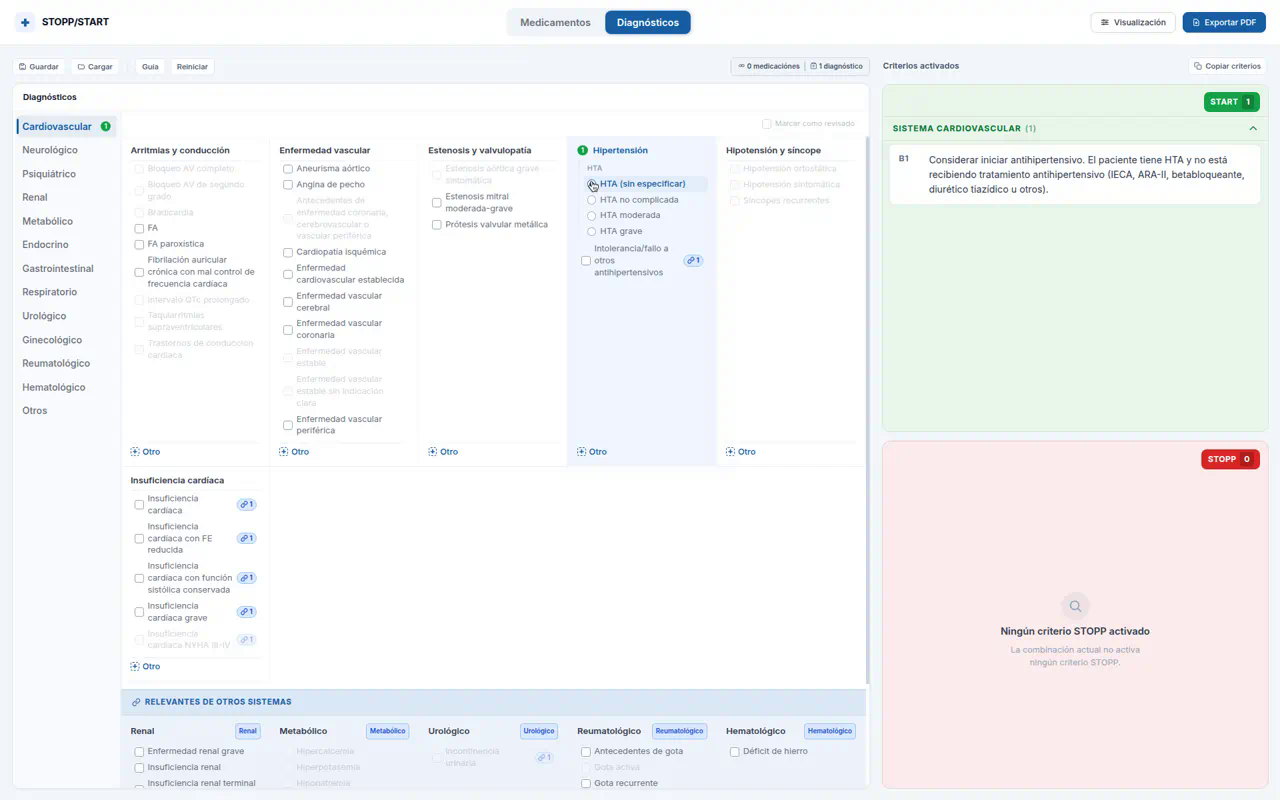
\includegraphics[width=\textwidth]{captura-hta-start-b1.png}
  \caption{Diagnósticos: HTA (sin especificar) marcada y criterio
    START-B1 activado. Ejecución del 01/09/2026 sobre el artefacto de
    producción.}
  \label{fig:cap-hta}
\end{figure}

\subsection{Pantalla de medicamentos}

La~\cref{fig:cap-amlodipino} muestra el primer paso: raíl de sistemas,
grupos propios y relevantes de otros sistemas, y el panel de avisos a la
derecha. Marcar un fármaco foráneo no duplica la selección; \emph{Otro}
añade un ítem con la clase del grupo. Cada pestaña vacía puede marcarse
como revisada.

\begin{figure}[H]
  \centering
  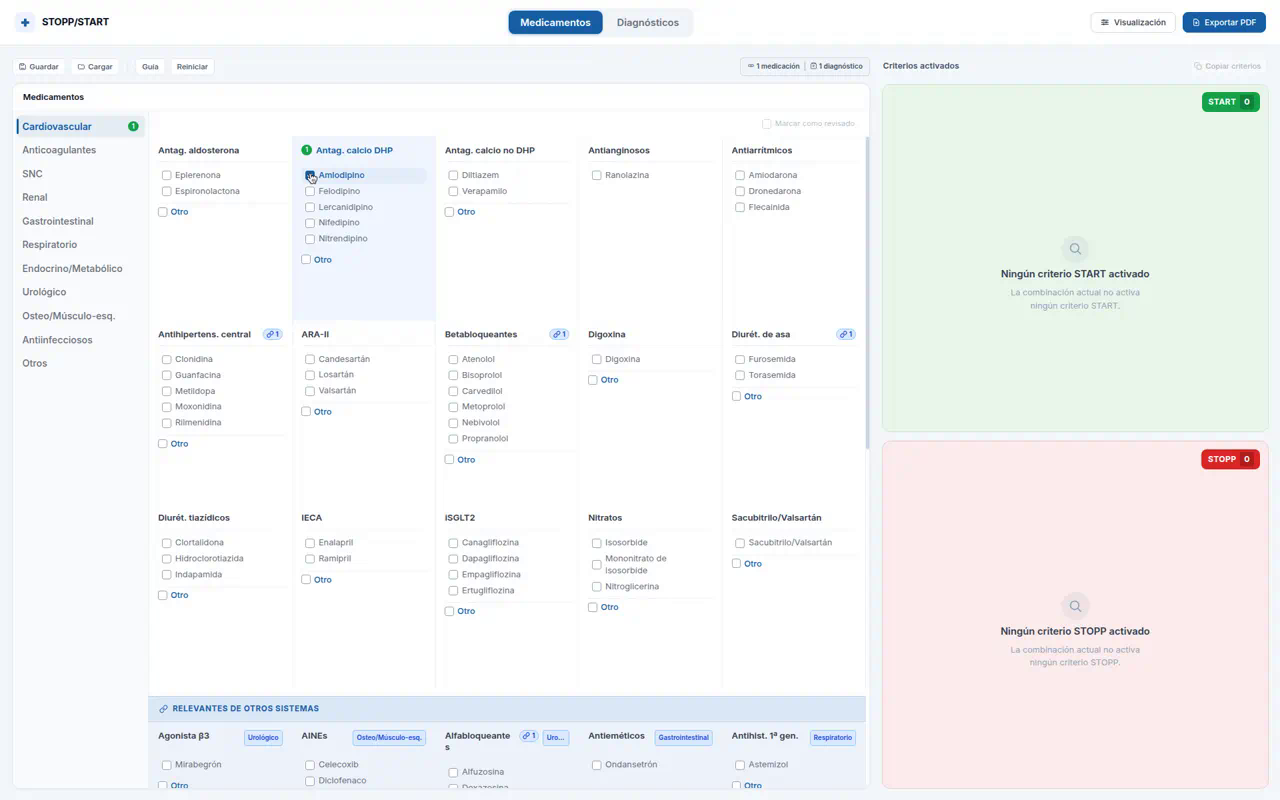
\includegraphics[width=\textwidth]{captura-amlodipino.png}
  \caption{Medicamentos: Amlodipino seleccionado; START-B1 deja de
    aplicar. Ejecución del 01/09/2026 sobre el artefacto de producción.}
  \label{fig:cap-amlodipino}
\end{figure}

\subsection{Pantalla de diagnósticos y analítica}

La~\cref{fig:cap-hta} muestra el segundo paso. Las familias como la
hipertensión son excluyentes. No hay ficha demográfica: la analítica
(TFGe, presión, frecuencia, QTc, iones, TSH) vive en la pestaña
\emph{Otros}; si un valor no se rellena, los criterios que lo leen no
disparan.

\subsection{Resultados y generación del informe}
\label{sec:resultados-manual}

El panel derecho (\cref{fig:cap-resultados}) es el resultado: no hay una
tercera pantalla. Los avisos START van encima; los STOPP, debajo. Cada
bloque muestra un contador y agrupa las tarjetas por sistema. El texto
de cada tarjeta es el \texttt{summary} del criterio; el profesional
juzga si aplican umbrales de dosis o duración.

\begin{figure}[H]
  \centering
  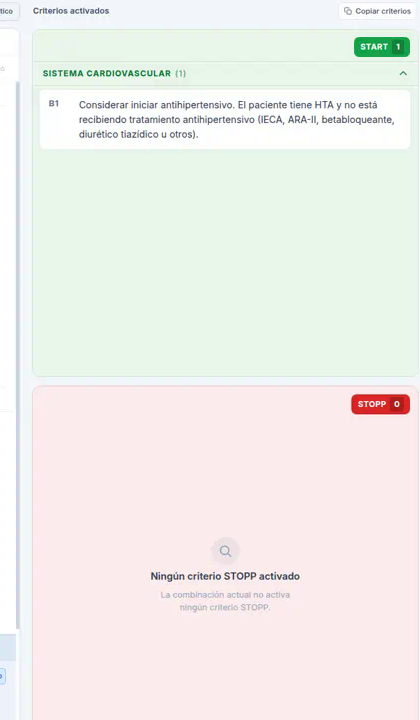
\includegraphics[height=0.26\textheight,keepaspectratio]{captura-resultados.png}
  \caption{Panel de criterios activados del caso HTA, con START-B1 y
    sin avisos STOPP. Detalle de la ejecución del 01/09/2026.}
  \label{fig:cap-resultados}
\end{figure}

Desde cualquier paso se puede exportar PDF, copiar criterios en texto
plano, guardar o cargar JSON v1.0 y reiniciar tras confirmación. Un JSON
ajeno o de versión distinta se rechaza con un mensaje comprensible.

\section{Resolución de errores}

La~\cref{tab:errores-manual} del~\cref{anexo:errores-uso} resume síntomas
de puesta en marcha, exportación y evaluación. No sustituye el
diagnóstico clínico cuando un criterio esperado no aparece.

\section{Preguntas frecuentes}

\paragraph{¿Esta herramienta sustituye al juicio clínico?}
No. Es un cribado: señala criterios STOPP/START que \emph{podrían}
aplicar al caso introducido. La decisión de deprescribir, iniciar o
mantener un tratamiento es siempre del profesional, a la luz de la
situación concreta y de la guía~\cite{omahony2023stopp,sacyl2023stopp}.

\paragraph{¿Dónde se guardan los datos?}
En el \texttt{localStorage} del navegador, en el origen desde el que se
sirve la página (en la ejecución documentada,
\texttt{127.0.0.1:4173}). No hay servidor de aplicación ni cuenta de
usuario. El contenido no sale del equipo salvo que se exporte un JSON o
un PDF.

\paragraph{¿Puedo cargar un caso ya revisado?}
Sí. \emph{Guardar} descarga un JSON v1.0; \emph{Cargar} lo restaura.
El fichero debe ser una exportación de esta aplicación.

        % 5.17
% =====================================================================
%  5.18 PRINCIPALES APORTACIONES
%  Rubrica: las aportaciones deben CORRESPONDERSE CON TODOS los
%  objetivos fijados en el capitulo 2. Repasa OE1, OE2... uno a uno.
% =====================================================================

\chapter{Principales aportaciones}
\label{cap:aportaciones}

\section{Cumplimiento de los objetivos}

% Tabla o recorrido explicito objetivo por objetivo. Es la forma mas
% directa de demostrar la correspondencia que pide la rubrica.

\begin{table}[H]
  \centering
  \begin{tabular}{@{}lp{9cm}@{}}
    \toprule
    \textbf{Objetivo} & \textbf{Aportación que lo cubre} \\
    \midrule
    OE1 &  \\
    OE2 &  \\
    \bottomrule
  \end{tabular}
  \caption{Correspondencia entre objetivos y aportaciones.}
  \label{tab:objetivos-aportaciones}
\end{table}

\section{Aportaciones técnicas}

\section{Aportaciones al ámbito clínico}
          % 5.18
% =====================================================================
%  5.19 CONCLUSIONES
%  Rubrica: hay que DIFERENCIAR CLARAMENTE las conclusiones tecnicas
%  de las personales. Mezclarlas baja la nota de forma explicita.
%  Por eso van en dos secciones separadas.
% =====================================================================

\chapter{Conclusiones}
\label{cap:conclusiones}

\section{Conclusiones técnicas}

Tres decisiones de diseño facilitaron el desarrollo documentado. La primera es
mantener las reglas de decisión fuera del código: el motor aplica
\texttt{criteria.json} en lugar de codificar STOPP/START v3 como
ramas de programa. Esa separación, descrita en
el~\cref{cap:arquitectura}, hizo posible auditar el cardiovascular
contra la guía~\cite{omahony2023stopp,sacyl2023stopp} y eliminar
criterios inventados o redundantes sin reescribir el evaluador.

La segunda es usar los tests como especificación ejecutable de la
interpretación realizada, no solo como red de seguridad del
software~\cite{beck2002tdd}. Formular un caso y su resultado esperado antes de
implementar la regla convirtió esa expectativa en un contrato comprobable. El
capítulo de pruebas separa el inventario estático de 985 cláusulas de su
resultado: la suite actual no se ha podido ejecutar en el entorno de cierre y,
por tanto, no se presenta como superada. También recoge las amenazas derivadas
de compartir interpretación entre regla y prueba y de no disponer de revisión
independiente completa.

La tercera es la arquitectura de página única sin servidor. En el
contexto de un TFG que maneja datos de salud, evaluar y persistir el
caso solo en el navegador evita un backend de pacientes y reduce la
exposición asociada a ese componente, aunque no elimina los riesgos del
almacenamiento local. El coste, aceptado en
el~\cref{cap:objetivos}, es no cubrir escenarios multiusuario ni
despliegue institucional.

Los límites técnicos son igual de concretos. El catálogo de fármacos y
diagnósticos está acotado a lo modelado: no cubre el arsenal terapéutico
completo. El modelo de datos admite edad y sexo, pero la interfaz no
ofrece un paso de ficha demográfica: esos campos solo llegan por
importación JSON. La analítica sí se captura en la pestaña «Otros» del paso de
diagnósticos. Así, la evaluación automática desde la UI se limita a
medicación, diagnósticos y esos valores; la importación JSON añade los datos
demográficos, aunque el catálogo actual solo consulta la edad; las condiciones
de dosis y duración exigen confirmación manual; y los criterios dependientes
de otros datos quedan sin evaluar. El recuento del catálogo (218 subcriterios
en \texttt{criteria.json}) no coincide 1:1 con los
190 enunciados de la guía: algunos se desglosan en varias reglas y no existe
una matriz que demuestre la correspondencia completa. Por último, las
dependencias diagnósticas y las familias de variantes se modelaron con mayor
detalle en cardiovascular e hipertensión; el resto de sistemas no tiene el
mismo grado de especialización.

\section{Conclusiones personales}

El trabajo se desarrolló con dos perfiles de tutoría distintos: el
tutor del área informática y la cotutora clínica. Esa dualidad obligó a
traducir de forma continua entre restricciones de software (alcance,
tests, interfaz) y matices de la guía. Cuando una duda clínica no
bloqueaba el desarrollo, se documentó y se siguió con la parte técnica;
cuando una petición de interfaz amenazaba el calendario, se dejó en
cuarentena en lugar de fusionarla. Ejemplos de ese filtro son el
historial de casos ---implementado y después eliminado--- y el selector
jerárquico de variantes, del que solo se incorporó la familia de
hipertensión.

Haría dos cosas de otro modo. La primera: registrar las horas desde el
primer día. La dedicación se ha reconstruido a posteriori a partir del
histórico de Git y de las rondas de trabajo, y esa reconstrucción es
menos precisa que un registro contemporáneo. La segunda: anteponer el
paso de datos del paciente (edad, sexo y constantes) a refinamientos de
la taxonomía. Varios criterios del motor ya dependían de esos campos
mientras la UI aún no permitía introducirlos; corregir ese desajuste
antes habría alineado el modelo, las pruebas y el flujo de entrada.

En conjunto, el proyecto muestra la importancia de acotar el alcance, hacer
comprobables las reglas y declarar de forma explícita lo que la evidencia
disponible todavía no permite sostener. Sin pacientes, revisión clínica
independiente completa ni evaluación formal de usabilidad, no se concluye
utilidad clínica ni mejora del trabajo en consulta.
          % 5.19
% =====================================================================
%  5.20 VIAS DE TRABAJO FUTURO
%  Rubrica: "presentadas con claridad". Lo que penaliza es que sean
%  "muy generales e inconcretas". Cada linea debe decir QUE falta,
%  POR QUE tiene sentido y QUE haria falta para abordarla.
% =====================================================================

\chapter{Vías de trabajo futuro}
\label{cap:futuro}

\section{Ampliación de la cobertura de criterios}

\section{Generalización de las dependencias entre diagnósticos}

% El trabajo pendiente de extender a todos los sistemas. Explicar que
% requiere primero generalizar la arquitectura y despues criterio
% clinico para rellenar los datos: eso lo hace concreto.

\section{Entrada en lenguaje natural y normalización con SNOMED CT}

% Linea de mayor recorrido. Explicar la idea, que aportaria y que
% dificultades tiene.

\section{Otras mejoras identificadas}
        % 5.20

% ---------- 5.21 Referencias ----------
\cleardoublepage
\phantomsection
\addcontentsline{toc}{chapter}{Referencias}
\printbibliography[title={Referencias}]

% ---------- 5.22 Anexos (opcionales, no cuentan para las 50 paginas) ----------
\appendix
% =====================================================================
%  5.22 ANEXOS (OPCIONALES)
%  No cuentan para el limite de 50 paginas: es el sitio para todo el
%  material voluminoso que en el cuerpo estorbaria.
%  main.tex ya ejecuta \appendix antes de este input.
% =====================================================================

\chapter{Comandos de operación}
\label{anexo:comandos}

Este anexo resume los comandos necesarios para instalar, ejecutar,
comprobar y auditar el prototipo desde la raíz del repositorio. El
recorrido de uso se describe en el~\cref{cap:manual}; aquí solo se
documenta la operación técnica. El servidor de desarrollo debe lanzarse
con la configuración \texttt{development}; no se emplea la
compilación de producción como entorno de trabajo.

\begin{table}[H]
  \centering
  \small
  \begin{tabularx}{\textwidth}{@{}>{\raggedright\ttfamily}p{7.4cm}X@{}}
    \toprule
    \textbf{\normalfont Comando} & \textbf{Propósito} \\
    \midrule
    npm install &
      Instala las dependencias declaradas en \texttt{package.json}. \\
    npx ng serve
    --host 127.0.0.1 --port 4200 &
      Arranca el servidor de desarrollo (configuración
      \texttt{development}) en el puerto 4200. \\
    npx ng test --watch=false
    --browsers=ChromeHeadless &
      Ejecuta la batería Karma + Jasmine en Chrome sin interfaz, una
      sola pasada. \\
    npx ng build
    --configuration development &
      Genera el artefacto de desarrollo (comprobación de tipos incluida). \\
    bash scripts/check-links.sh &
      Verifica el patrón de documentación enlazada (\texttt{@linked}):
      enlaces rotos, documentos huérfanos y ficheros fuera del mapa. \\
    node scripts/audit-criteria.cjs &
      Audita la consistencia entre \texttt{criteria.json}, el catálogo
      de fármacos y el de diagnósticos (clases y códigos huérfanos). \\
    \bottomrule
  \end{tabularx}
  \caption{Comandos de instalación, ejecución, prueba y auditoría.}
  \label{tab:comandos-operacion}
\end{table}

El script \texttt{scripts/check-links.sh} existe en el repositorio y
debe terminar con código de salida 0. Las líneas de consola del tipo
«Error evaluando criterio» que puedan aparecer durante
\texttt{ng test} corresponden a una especificación deliberada de manejo
de errores, no a un fallo de la suite: el veredicto es la línea final
de totales.

\chapter{Sistemas clínicos y recuento de criterios}
\label{anexo:sistemas}

La guía STOPP/START v3 formula 190 enunciados (133 STOPP y 57
START)~\cite{omahony2023stopp}. El catálogo de la aplicación no los
reproduce 1:1: algunos enunciados se desglosan en varias reglas
(subcriterios) y otros se agrupan. La~\cref{tab:sistemas-criterios}
resume, por los 13 sistemas del fichero \texttt{criteria.json}, cuántas
reglas STOPP y START hay implementadas. No se listan los textos
completos: el volumen duplicaría la memoria sin añadir información de
diseño.

Los recuentos corresponden a la versión del catálogo presente en el corte
documental del 16 de agosto de 2026 (218 reglas: 166 STOPP y 52 START). Son cifras de
implementación, no un censo de la guía impresa~\cite{sacyl2023stopp}.

\begin{table}[H]
  \centering
  \small
  \begin{tabular}{@{}lrrr@{}}
    \toprule
    \textbf{Sistema clínico} & \textbf{STOPP} & \textbf{START} & \textbf{Total} \\
    \midrule
    Indicación de la medicación                    &   8 &  0 &   8 \\
    Sistema cardiovascular                         &  35 & 11 &  46 \\
    Anticoagulantes/Antiagregantes                 &  19 &  2 &  21 \\
    Sistema nervioso central                       &  31 &  7 &  38 \\
    Sistema renal                                  &  10 &  4 &  14 \\
    Sistema gastrointestinal                       &   9 &  7 &  16 \\
    Sistema respiratorio                           &   4 &  3 &   7 \\
    Sistema musculoesquelético                     &  11 &  9 &  20 \\
    Sistema urogenital                             &   8 &  5 &  13 \\
    Sistema endocrino                              &  11 &  1 &  12 \\
    Riesgo de caídas                               &  14 &  0 &  14 \\
    Analgésicos                                    &   5 &  3 &   8 \\
    Carga antimuscarínica/anticolinérgica          &   1 &  0 &   1 \\
    \midrule
    \textbf{Total}                                 & \textbf{166} & \textbf{52} & \textbf{218} \\
    \bottomrule
  \end{tabular}
  \caption{Reglas implementadas por sistema clínico (catálogo
    \texttt{criteria.json}).}
  \label{tab:sistemas-criterios}
\end{table}

\chapter{Trazabilidad entre requisitos y evidencia}
\label{anexo:trazabilidad}

La~\cref{tab:trazabilidad-requisitos} enlaza cada requisito con evidencia
localizada en el repositorio. «Localizada» significa que existe una
especificación automática que expresa ese comportamiento; no significa que
la suite se haya ejecutado con éxito para esta edición de la memoria.
«Parcial» identifica requisitos cuya dimensión completa exige medición,
auditoría o prueba de uso adicional. Salvo las rutas que comienzan por
\texttt{src/}, los nombres de fichero se refieren a \texttt{src/app/}.

{\scriptsize
\begin{longtable}{@{}p{0.7cm}p{3.4cm}p{6.0cm}p{2.7cm}@{}}
  \caption{Matriz requisitos--evidencia del repositorio.}
  \label{tab:trazabilidad-requisitos} \\
  \toprule
  \textbf{ID} & \textbf{Comportamiento trazado} &
  \textbf{Evidencia localizada} & \textbf{Estado documental} \\
  \midrule
  \endfirsthead
  \caption[]{Matriz requisitos--evidencia del repositorio (cont.).} \\
  \toprule
  \textbf{ID} & \textbf{Comportamiento trazado} &
  \textbf{Evidencia localizada} & \textbf{Estado documental} \\
  \midrule
  \endhead
  \bottomrule
  \endfoot
  RF01 & Seleccionar y deseleccionar medicamentos &
    \texttt{steps/meds-step/meds-step.component.spec.ts};
    \texttt{core/group-checked.spec.ts} &
    Localizada; ejecución final no registrada \\
  RF02 & Seleccionar diagnósticos y variantes excluyentes &
    \texttt{steps/diagnosis-step/diagnosis-step.component.spec.ts};
    \texttt{core/data/diagnosis-variants.spec.ts} &
    Localizada; ejecución final no registrada \\
  RF03 & Capturar analítica y constantes &
    \texttt{core/lab-capture.spec.ts};
    \texttt{steps/diagnosis-step/diagnosis-step.component.spec.ts} &
    Localizada; ejecución final no registrada \\
  RF04 & Reevaluar tras cambios del caso &
    \texttt{core/services/criteria-engine.service.spec.ts};
    especificaciones de ambos pasos &
    Localizada; ejecución final no registrada \\
  RF05 & Calcular advertencias preventivas de medicación &
    \texttt{core/services/criteria-engine.service.spec.ts} &
    Solo motor; no integrado en la interfaz; ejecución final no registrada \\
  RF06 & Mostrar elementos relevantes de otros sistemas &
    \texttt{core/data/system-relevance.spec.ts};
    \texttt{core/group-visibility.spec.ts} &
    Localizada; ejecución final no registrada \\
  RF07 & Marcar pestañas revisadas y persistir el estado &
    \texttt{core/case-store.service.spec.ts} &
    Localizada; ejecución final no registrada \\
  RF08 & Agrupar resultados por tipo y sistema &
    \texttt{core/criteria-groups.spec.ts};
    especificaciones de ambos pasos &
    Localizada; ejecución final no registrada \\
  RF09 & Generar y descargar el informe PDF &
    \texttt{core/report.service.spec.ts} &
    Localizada; no se adjunta PDF ejecutado \\
  RF10 & Copiar criterios como texto plano &
    \texttt{core/clipboard-text.spec.ts};
    especificaciones de ambos pasos &
    Localizada; ejecución final no registrada \\
  RF11 & Exportar e importar JSON validado &
    \texttt{core/case-io.service.spec.ts} &
    Localizada; no se adjunta JSON ejecutado \\
  RF12 & Reiniciar solo tras confirmación &
    \texttt{confirm-reset-dialog.component.spec.ts};
    \texttt{core/case-store.service.spec.ts} &
    Localizada; ejecución final no registrada \\
  RF13 & Escala de fuente y orientación persistentes &
    \texttt{core/display-settings.service.spec.ts};
    especificaciones de ambos pasos &
    Localizada; ejecución final no registrada \\
  RF14 & Guía rápida y enlace a la guía oficial &
    \texttt{quick-guide-dialog.component.spec.ts} &
    Localizada; ejecución final no registrada \\
  RF15 & Opción «Otro» por grupo &
    \texttt{core/group-checked.spec.ts};
    especificaciones de ambos pasos &
    Localizada; ejecución final no registrada \\
  RNF01 & Flujo en dos pasos con resultados junto a la captura &
    \texttt{app.routes.spec.ts}; especificaciones de ambos pasos &
    Parcial: estructura localizada; usabilidad no evaluada \\
  RNF02 & Evaluación en cliente en la misma interacción &
    \texttt{core/services/criteria-engine.service.spec.ts};
    especificaciones de ambos pasos &
    Parcial: sin medición de latencia \\
  RNF03 & Tres escalas de fuente &
    \texttt{core/display-settings.service.spec.ts} &
    Parcial: sin auditoría de accesibilidad \\
  RNF04 & Catálogo JSON separado del motor &
    \texttt{src/assets/data/criteria.json};
    \texttt{core/data/criteria-data-integrity.spec.ts} &
    Estructura localizada; ejecución final no registrada \\
  RNF05 & Persistencia local del caso &
    \texttt{core/case-store.service.spec.ts};
    \texttt{core/case-io.service.spec.ts} &
    Parcial: persistencia localizada; privacidad no auditada \\
\end{longtable}
}

\chapter{Cobertura demostrable del catálogo de criterios}
\label{anexo:cobertura-criterios}

El catálogo contiene 218 reglas JSON, distribuidas como muestra la
\cref{tab:sistemas-criterios}. Ese recuento se obtiene directamente de
\texttt{src/assets/data/criteria.json}. Las especificaciones
\texttt{criteria-a.spec.ts} a \texttt{criteria-m.spec.ts} contienen casos
por secciones del catálogo, y
\texttt{criteria-data-integrity.spec.ts} expresa guardas entre reglas y
catálogos.

La~\cref{tab:cobertura-catalogo} es deliberadamente una matriz de
\emph{evidencia del repositorio}, no una matriz de equivalencia clínica.
La presencia de un fichero por sección tampoco demuestra por sí sola que
cada una de sus reglas tenga casos positivo y negativo ejecutados.
No se ha validado una correspondencia criterio por criterio entre los 190
enunciados de la guía (133 STOPP y 57 START) y las 218 reglas. Una regla
puede desglosar parte de un enunciado, varias reglas pueden agruparse o un
criterio puede necesitar datos no capturados. Por tanto, ningún recuento de
esta tabla demuestra cobertura completa de la guía.

{\scriptsize
\begin{longtable}{@{}p{4.5cm}rrp{3.0cm}p{3.0cm}@{}}
  \caption{Matriz de cobertura demostrable del catálogo, sin equivalencia
  190$\rightarrow$218.}
  \label{tab:cobertura-catalogo} \\
  \toprule
  \textbf{Sistema del catálogo} & \textbf{STOPP} & \textbf{START} &
  \textbf{Especificación localizada} & \textbf{Correspondencia con guía} \\
  \midrule
  \endfirsthead
  \caption[]{Matriz de cobertura demostrable del catálogo (cont.).} \\
  \toprule
  \textbf{Sistema del catálogo} & \textbf{STOPP} & \textbf{START} &
  \textbf{Especificación localizada} & \textbf{Correspondencia con guía} \\
  \midrule
  \endhead
  \bottomrule
  \endfoot
  Indicación de la medicación & 8 & 0 & \texttt{criteria-a.spec.ts} & No validada \\
  Sistema cardiovascular & 35 & 11 & \texttt{criteria-b.spec.ts} & No validada \\
  Anticoagulantes/Antiagregantes & 19 & 2 & \texttt{criteria-c.spec.ts} & No validada \\
  Sistema nervioso central & 31 & 7 & \texttt{criteria-d.spec.ts} & No validada \\
  Sistema renal & 10 & 4 & \texttt{criteria-e.spec.ts} & No validada \\
  Sistema gastrointestinal & 9 & 7 & \texttt{criteria-f.spec.ts} & No validada \\
  Sistema respiratorio & 4 & 3 & \texttt{criteria-g.spec.ts} & No validada \\
  Sistema musculoesquelético & 11 & 9 & \texttt{criteria-h.spec.ts} & No validada \\
  Sistema urogenital & 8 & 5 & \texttt{criteria-i.spec.ts} & No validada \\
  Sistema endocrino & 11 & 1 & \texttt{criteria-j.spec.ts} & No validada \\
  Riesgo de caídas & 14 & 0 & \texttt{criteria-k.spec.ts} & No validada \\
  Analgésicos & 5 & 3 & \texttt{criteria-l.spec.ts} & No validada \\
  Carga antimuscarínica/anticolinérgica & 1 & 0 &
    \texttt{criteria-m.spec.ts} & No validada \\
  \midrule
  \textbf{Total del catálogo} & \textbf{166} & \textbf{52} &
    \textbf{Especificaciones localizadas; ejecución final no registrada} &
    \textbf{No validada} \\
\end{longtable}
}

Para convertir esta matriz en una acreditación de cobertura clínica falta
una revisión independiente que enumere los 190 criterios oficiales y, para
cada uno, identifique reglas, datos necesarios, caso positivo, caso
negativo y estado (completo, parcial, manual, no evaluable o no
implementado). Esa correspondencia no puede inferirse de los totales y no
se inventa en esta memoria.


\end{document}
